%%%%%%%%%%%%%%%%%%%%%%%%%%%%%%%%%%%%%%%%%
% Beamer Presentation
% LaTeX Template
% Version 1.0 (10/11/12)
%
% This template has been downloaded from:
% http://www.LaTeXTemplates.com
%
% License:
% CC BY-NC-SA 3.0 (http://creativecommons.org/licenses/by-nc-sa/3.0/)
%
%%%%%%%%%%%%%%%%%%%%%%%%%%%%%%%%%%%%%%%%%

%----------------------------------------------------------------------------------------
%    PACKAGES AND THEMES
%----------------------------------------------------------------------------------------

\documentclass[usenames,dvipsnames]{beamer}
\usepackage{animate}
\usepackage{float}
\usepackage{bm}
\usepackage{mathtools}
\usepackage{extarrows}
\usepackage{ctex}
\usepackage[T1]{fontenc}
\usepackage{beramono}
\usepackage{listings}
\usepackage{xcolor}

%%
%% Julia definition (c) 2014 Jubobs
%%
\lstdefinelanguage{Julia}%
  {morekeywords={abstract,break,case,catch,const,continue,do,else,elseif,%
      end,export,false,for,function,immutable,import,importall,if,in,%
      macro,module,otherwise,quote,return,switch,true,try,type,typealias,%
      using,while},%
   sensitive=true,%
   morecomment=[l]\#,%
   morecomment=[n]{\#=}{=\#},%
   morestring=[s]{"}{"},%
   morestring=[m]{'}{'},%
}[keywords,comments,strings]%

\lstset{%
    language         = Julia,
    basicstyle       = \ttfamily,
    keywordstyle     = \bfseries\color{blue},
    stringstyle      = \color{magenta},
    commentstyle     = \color{ForestGreen},
    showstringspaces = false,
}
\newcommand{\ChoL}{\mathsf{L}}
\newcommand{\bx}{\mathbf{x}}
\newcommand{\ii}{\mathrm{i}}
\newcommand{\bxi}{\bm{\xi}}
\newcommand{\bmu}{\bm{\mu}}
\newcommand{\bb}{\mathbf{b}}
\newcommand{\bA}{\mathbf{A}}
\newcommand{\bJ}{\mathbf{J}}
\newcommand{\bB}{\mathbf{B}}
\newcommand{\bM}{\mathbf{M}}

\newcommand{\by}{\mathbf{y}}
\newcommand{\bw}{\mathbf{w}}

\newcommand{\bX}{\mathbf{X}}
\newcommand{\bY}{\mathbf{Y}}
\newcommand{\bs}{\mathbf{s}}
\newcommand{\sign}{\mathrm{sign}}
\newcommand{\bt}[0]{\bm{\theta}}
\newcommand{\bc}{\mathbf{c}}
\newcommand{\bzero}{\mathbf{0}}
\renewcommand{\bf}{\mathbf{f}}
\newcommand{\bu}{\mathbf{u}}
\newcommand{\bv}[0]{\mathbf{v}}

\mode<presentation> {

% The Beamer class comes with a number of default slide themes
% which change the colors and layouts of slides. Below this is a list
% of all the themes, uncomment each in turn to see what they look like.

%\usetheme{default}
%\usetheme{AnnArbor}
%\usetheme{Antibes}
%\usetheme{Bergen}
%\usetheme{Berkeley}
%\usetheme{Berlin}
%\usetheme{Boadilla}
%\usetheme{CambridgeUS}
%\usetheme{Copenhagen}
%\usetheme{Darmstadt}
%\usetheme{Dresden}
%\usetheme{Frankfurt}
%\usetheme{Goettingen}
%\usetheme{Hannover}
%\usetheme{Ilmenau}
%\usetheme{JuanLesPins}
%\usetheme{Luebeck}
\usetheme{Madrid}
%\usetheme{Malmoe}
%\usetheme{Marburg}
%\usetheme{Montpellier}
%\usetheme{PaloAlto}
%\usetheme{Pittsburgh}
%\usetheme{Rochester}
%\usetheme{Singapore}
%\usetheme{Szeged}
%\usetheme{Warsaw}


% As well as themes, the Beamer class has a number of color themes
% for any slide theme. Uncomment each of these in turn to see how it
% changes the colors of your current slide theme.

%\usecolortheme{albatross}
\usecolortheme{beaver}
%\usecolortheme{beetle}
%\usecolortheme{crane}
%\usecolortheme{dolphin}
%\usecolortheme{dove}
%\usecolortheme{fly}
%\usecolortheme{lily}
%\usecolortheme{orchid}
%\usecolortheme{rose}
%\usecolortheme{seagull}
%\usecolortheme{seahorse}
%\usecolortheme{whale}
%\usecolortheme{wolverine}

%\setbeamertemplate{footline} % To remove the footer line in all slides uncomment this line
%\setbeamertemplate{footline}[page number] % To replace the footer line in all slides with a simple slide count uncomment this line

%\setbeamertemplate{navigation symbols}{} % To remove the navigation symbols from the bottom of all slides uncomment this line
}
\usepackage{booktabs}
\usepackage{makecell}

\usepackage{soul}
\newcommand{\red}[1]{\textcolor{red}{#1}}
%
%\usepackage{graphicx} % Allows including images
%\usepackage{booktabs} % Allows the use of \toprule, \midrule and \bottomrule in tables
%
%
%\usepackage{amsthm}
%
%\usepackage{todonotes}
%\usepackage{floatrow}
%
%\usepackage{pgfplots,algorithmic,algorithm}
\usepackage{algorithmicx}
\usepackage{algpseudocode}
%\usepackage[toc,page]{appendix}
%\usepackage{float}
%\usepackage{booktabs}
%\usepackage{bm}
%
%\theoremstyle{definition}
%
\newcommand{\RR}[0]{\mathbb{R}}
%
%\newcommand{\bx}{\mathbf{x}}
%\newcommand{\ii}{\mathrm{i}}
%\newcommand{\bxi}{\bm{\xi}}
%\newcommand{\bmu}{\bm{\mu}}
%\newcommand{\bb}{\mathbf{b}}
%\newcommand{\bA}{\mathbf{A}}
%\newcommand{\bJ}{\mathbf{J}}
%\newcommand{\bB}{\mathbf{B}}
%\newcommand{\bM}{\mathbf{M}}
%\newcommand{\bF}{\mathbf{F}}
%
%\newcommand{\by}{\mathbf{y}}
%\newcommand{\bw}{\mathbf{w}}
%\newcommand{\bn}{\mathbf{n}}
%
%\newcommand{\bX}{\mathbf{X}}
%\newcommand{\bY}{\mathbf{Y}}
%\newcommand{\bs}{\mathbf{s}}
%\newcommand{\sign}{\mathrm{sign}}
%\newcommand{\bt}[0]{\bm{\theta}}
%\newcommand{\bc}{\mathbf{c}}
%\newcommand{\bzero}{\mathbf{0}}
%\renewcommand{\bf}{\mathbf{f}}
%\newcommand{\bu}{\mathbf{u}}
%\newcommand{\bv}[0]{\mathbf{v}}

\AtBeginSection[]
{
   \begin{frame}
       \frametitle{Outline}
       \tableofcontents[currentsection]
   \end{frame}
}

%----------------------------------------------------------------------------------------
%    TITLE PAGE
%----------------------------------------------------------------------------------------
\usepackage{bm}
\newcommand*{\TakeFourierOrnament}[1]{{%
\fontencoding{U}\fontfamily{futs}\selectfont\char#1}}
\newcommand*{\danger}{\TakeFourierOrnament{66}}

\title[Physics Based Machine Learning]{ADCME.jl \\ {Physics Based Machine Learning for Inverse Problems}} % The short title appears at the bottom of every slide, the full title is only on the title page

\author[ADCME]{Kailai Xu (许开来)\\\url{https://github.com/kailaix/ADCME.jl}} % Your name
%\institute[] % Your institution as it will appear on the bottom of every slide, may be shorthand to save space
%{
%%ICME, Stanford University \\ % Your institution for the title page
%%\medskip
%%\textit{kailaix@stanford.edu}\quad \textit{darve@stanford.edu} % Your email address
%}
\date{}% Date, can be changed to a custom date
% Mathematics of PDEs


\begin{document}

\usebackgroundtemplate{%
\begin{picture}(0,250)
\centering
	{{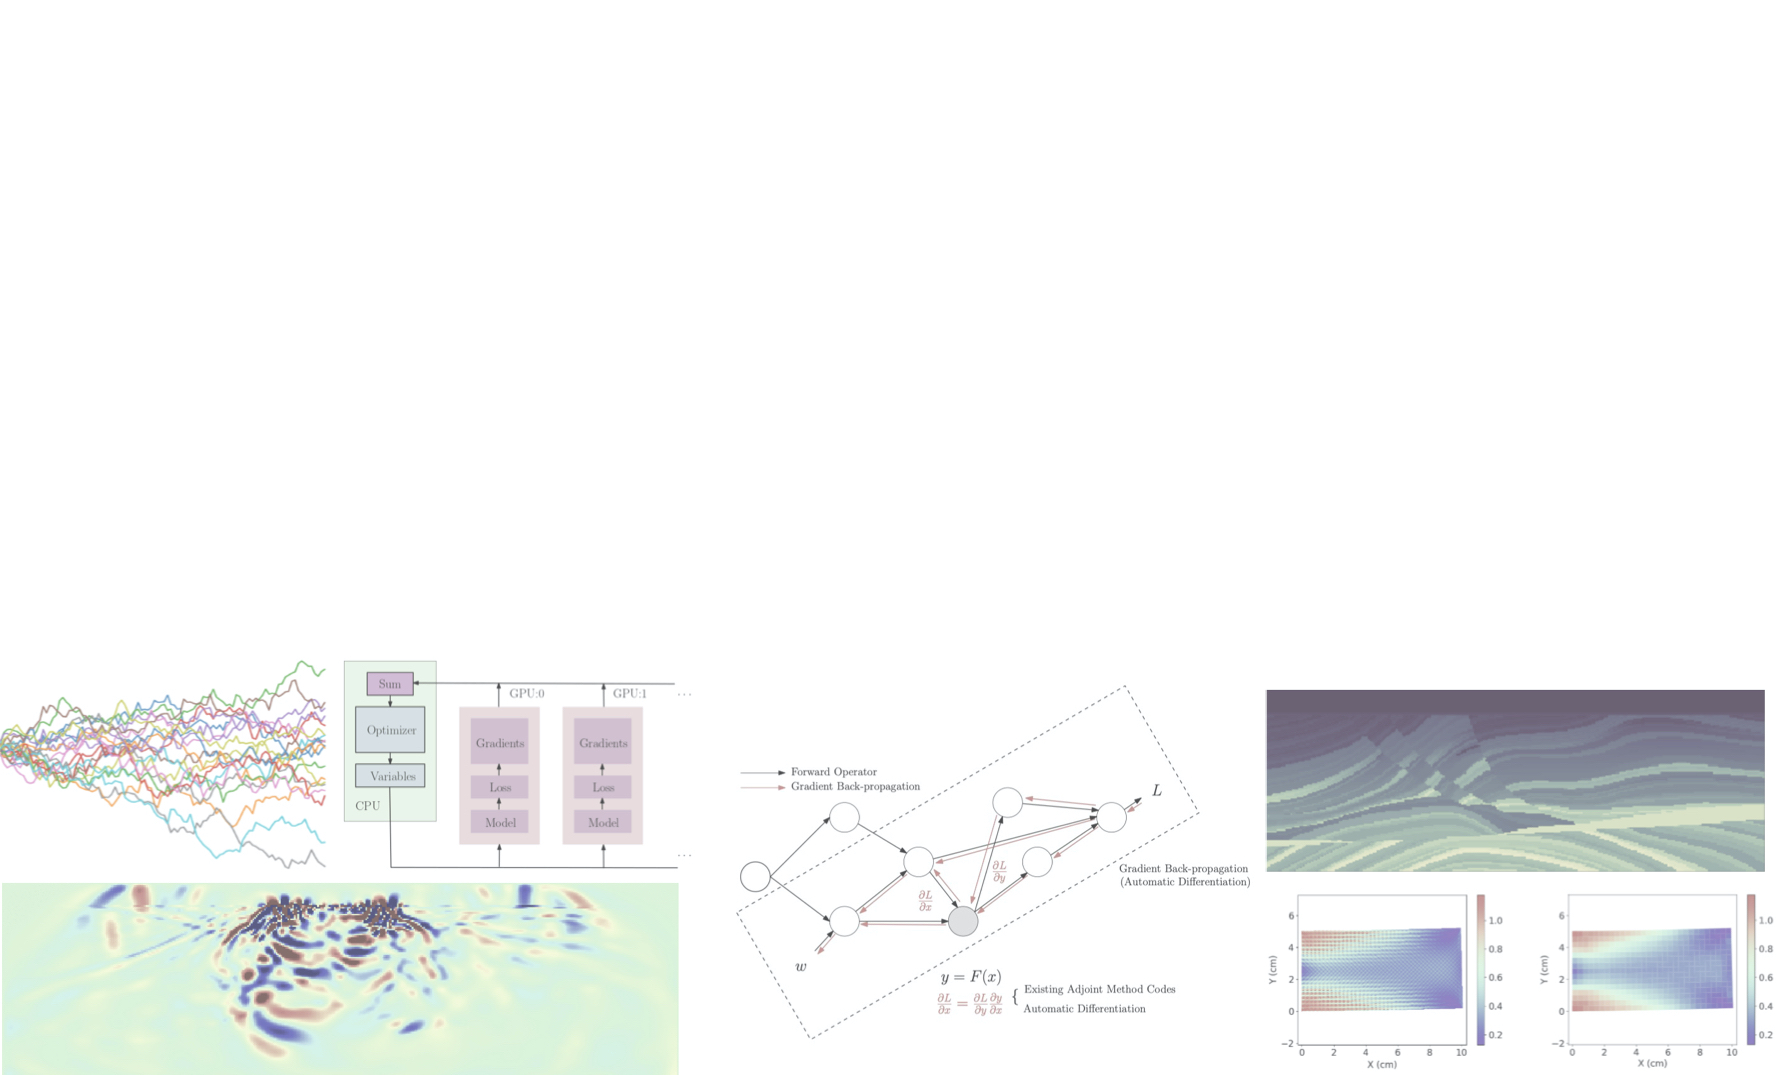
\includegraphics[width=1.0\paperwidth]{figures/background}}}
\end{picture}
  } 
%\usebackgroundtemplate{%
%  \includegraphics[width=\paperwidth,height=\paperheight]{figures/back}} 
\begin{frame}

\titlepage % Print the title page as the first slide

%dfa
\end{frame}
\usebackgroundtemplate{}




\begin{frame}
	This work (ADCME.jl and its ecosystem) is a result of collective efforts of many of my Ph.D. collaborators together with our faculty advisors. In \textcolor{red}{chronological order} they are:
	
	\begin{itemize}
		\item Ph.D. collaborators: Daniel (Zhengyu) Huang, Dongzhuo Li, Weiqiang Zhu, and Tiffany (Li) Fan. 
		\item Faculty supervisors: Eric Darve, Charbel Farhat, Jerry M. Harris, and Gregory C. Beroza. 
		\item Many other fellow researchers from Julia language and scientific computing communities, who provide valuable inputs. 
	\end{itemize}
\end{frame}



\section{Inverse Modeling}



\begin{frame}
	\frametitle{Inverse Modeling}
	\begin{itemize}
		\item \textbf{Inverse modeling} (逆建模) identifies a certain set of parameters or functions with which the outputs of the forward analysis matches the desired result or measurement.
		\item Many real life engineering problems can be formulated as inverse modeling problems: shape optimization for improving the performance of structures, optimal control of fluid dynamic systems, etc.
	\end{itemize}
	\begin{figure}[hbt]
	\centering
  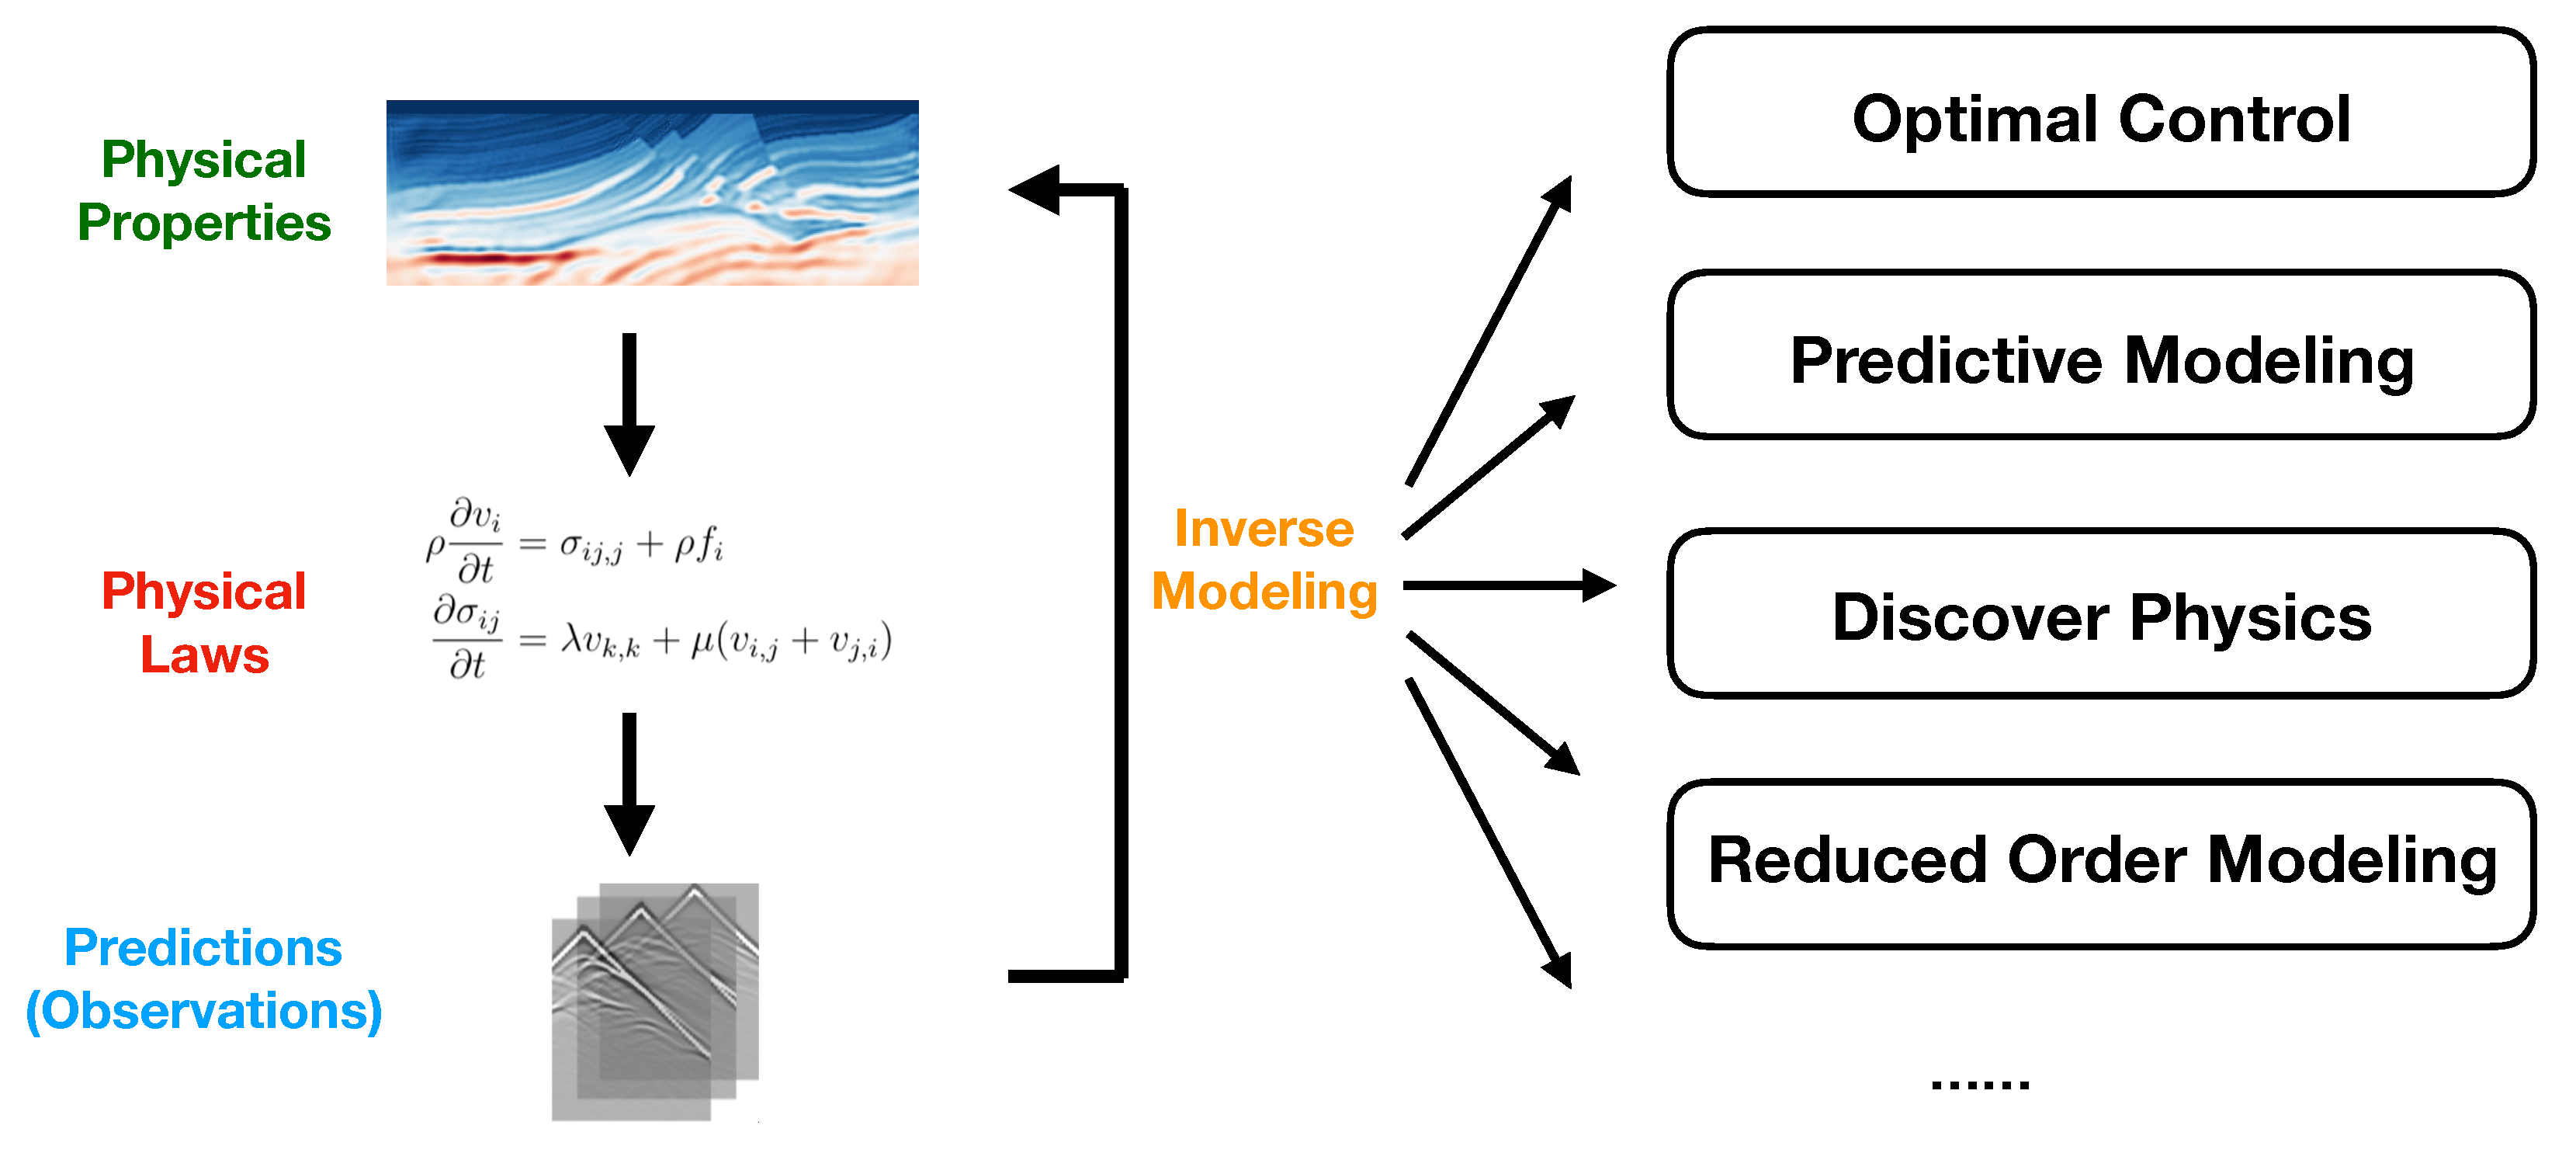
\includegraphics[width=0.8\textwidth]{figures/inverse2}
\end{figure}
\end{frame}

\begin{frame}
	\frametitle{Inverse Modeling}
	\begin{figure}
	\centering
  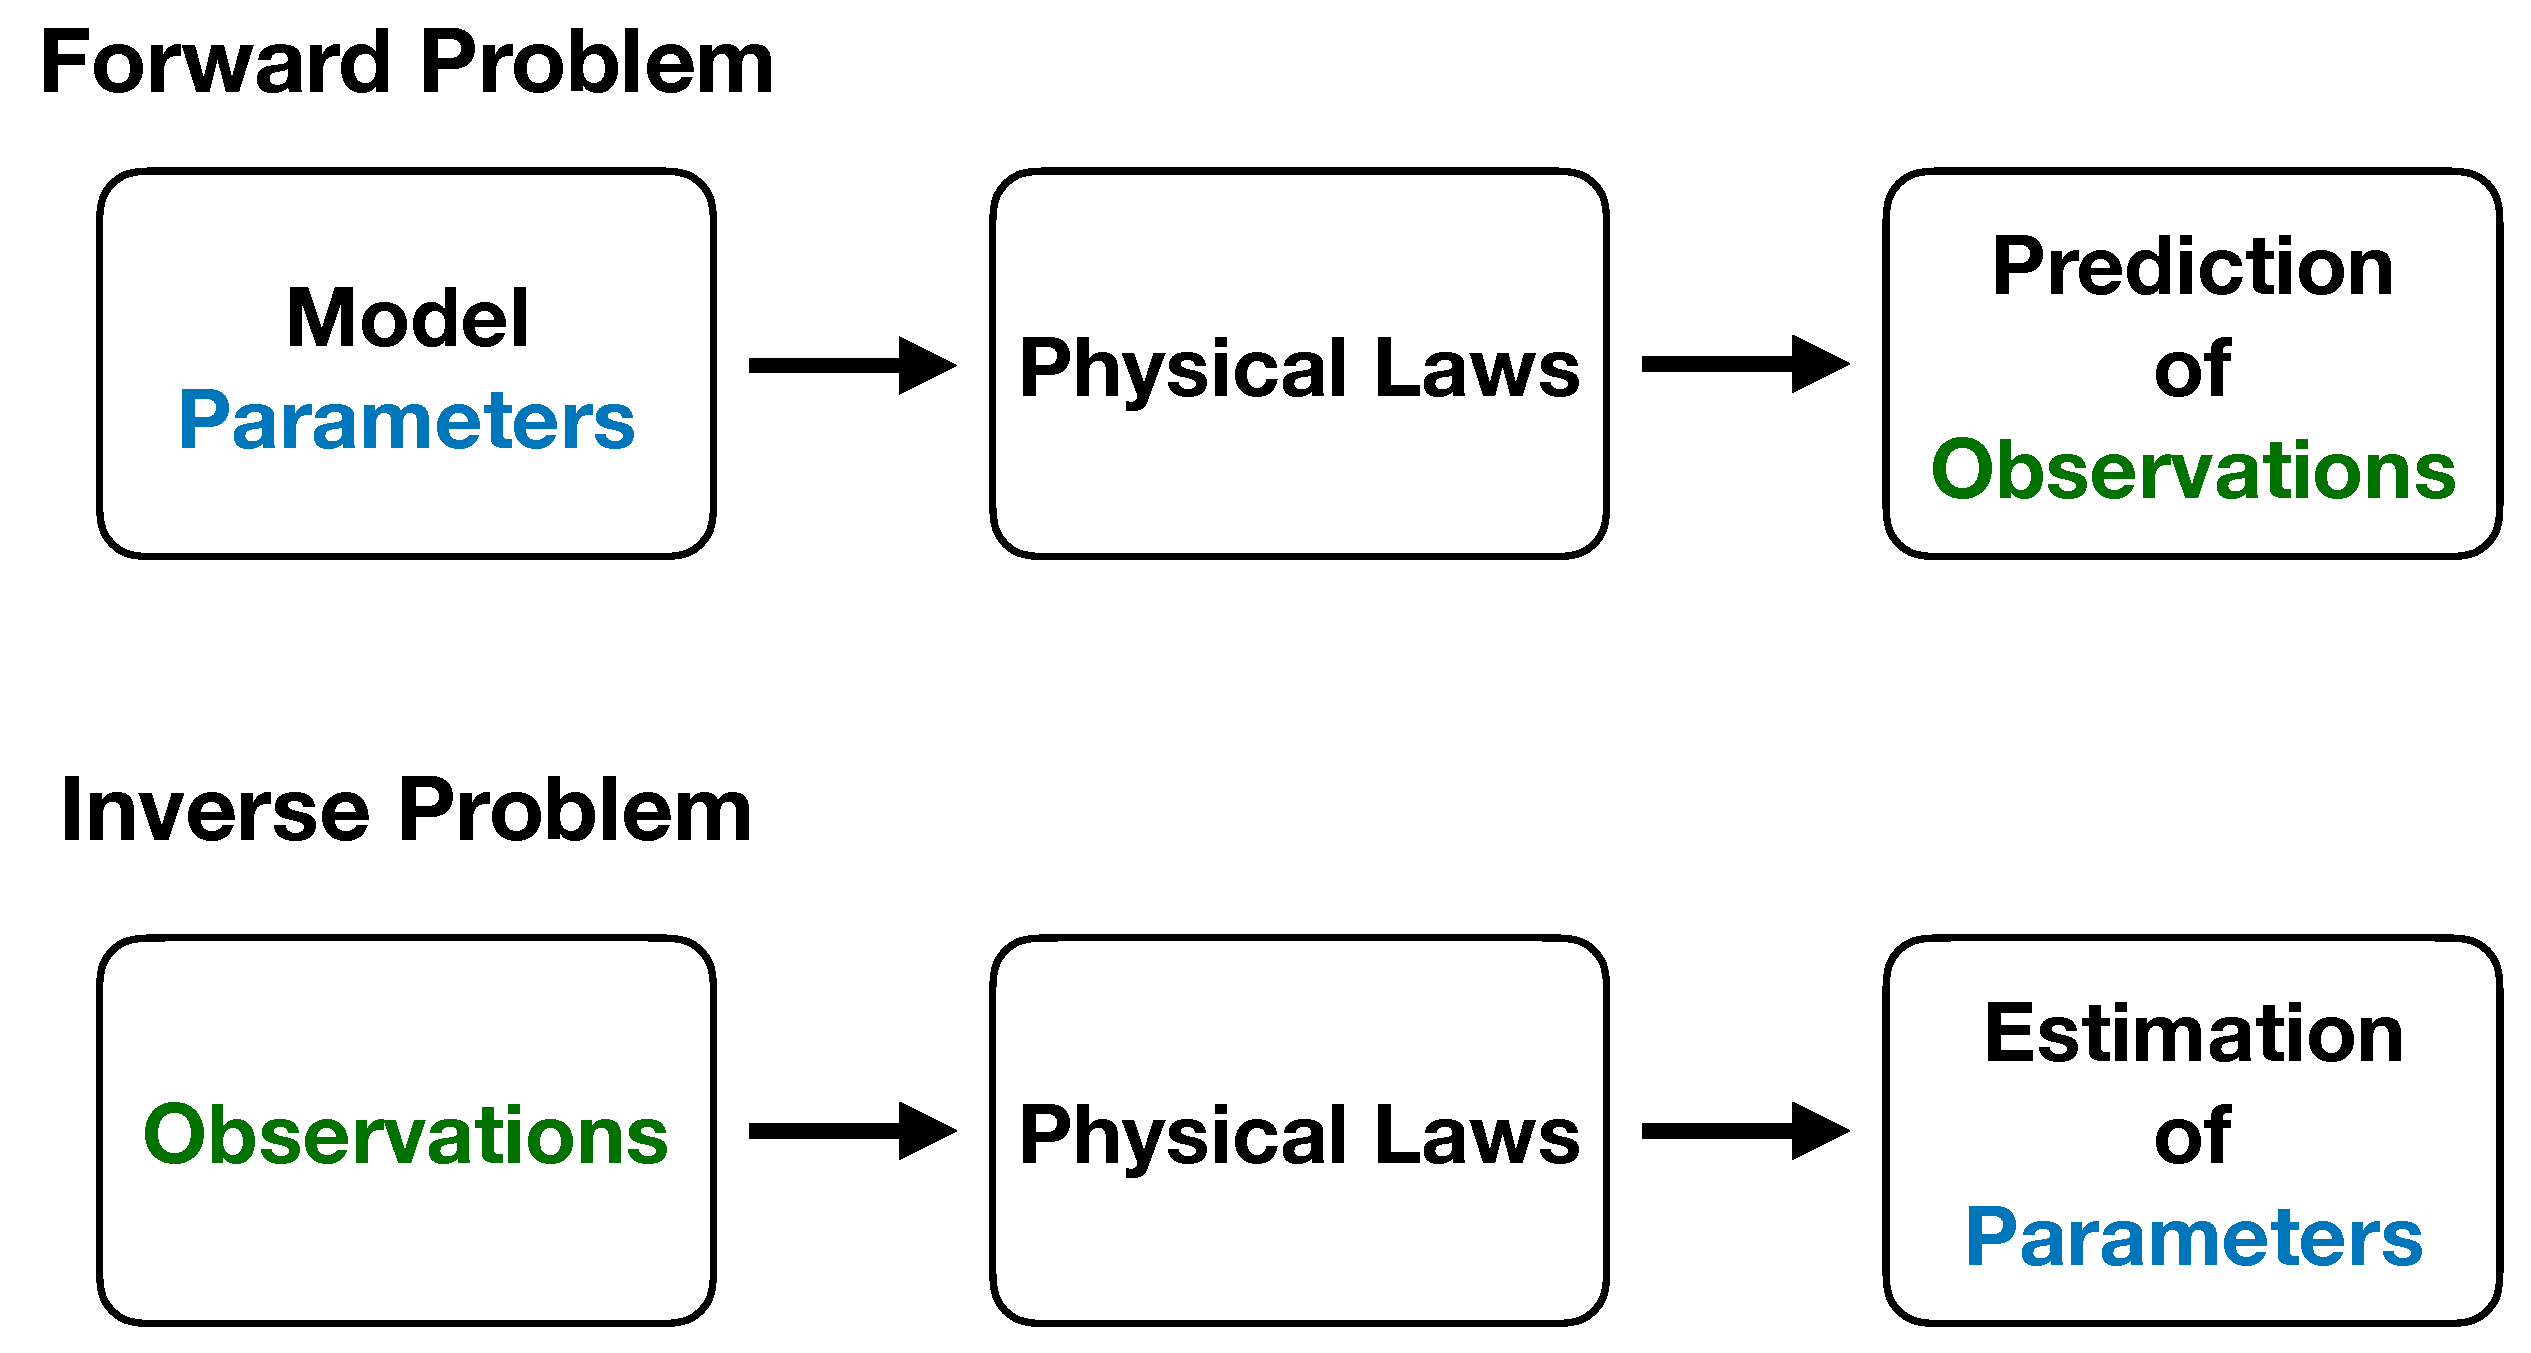
\includegraphics[width=1.0\textwidth]{figures/inverse3}
\end{figure}
\end{frame}

\begin{frame}
	\frametitle{Inverse Modeling}
	We can formulate inverse modeling as a PDE-constrained optimization problem 
	\begin{equation*}
		\min_{\theta} L_h(u_h) \quad \mathrm{s.t.}\; F_h(\theta, u_h) = 0
	\end{equation*}
	\begin{itemize}
		\item The \textcolor{red}{loss function} $L_h$ measures the discrepancy between the prediction $u_h$ and the observation $u_{\mathrm{obs}}$, e.g., $L_h(u_h) = \|u_h - u_{\mathrm{obs}}\|_2^2$. 
		\item $\theta$ is the \textcolor{red}{model parameter} to be calibrated. 
		\item The \textcolor{red}{physics constraints} $F_h(\theta, u_h)=0$ are described by a system of partial differential equations. Solving for $u_h$ may require solving linear systems or applying an iterative algorithm such as the Newton-Raphson method. 
	\end{itemize}
\end{frame}

\begin{frame}
	\frametitle{Function Inverse Problem}
	
	\begin{equation*}
		\min_{\textcolor{red}{f}} L_h(u_h) \quad \mathrm{s.t.}\; F_h(\textcolor{red}{f}, u_h) = 0
	\end{equation*}
	
	What if the unknown is a \textcolor{red}{function} instead of a set of parameters?
\begin{itemize}
	\item Koopman operator in dynamical systems.
	\item Constitutive relations in solid mechanics. 
	\item Turbulent closure relations in fluid mechanics.
	\item ...
\end{itemize}

The candidate solution space is \textcolor{red}{infinite dimensional}.

\end{frame}

\begin{frame}
	\frametitle{Physics Based Machine Learning}
	$$\min_{\theta} L_h(u_h) \quad \mathrm{s.t.}\;F_h(\textcolor{red}{NN_\theta}, u_h) = 0$$
	\vspace{-0.5cm}
	\begin{itemize}
		\item Deep neural networks exhibit capability of approximating high dimensional and complicated functions. 
		\item \textbf{Physics based machine learning}: \textcolor{red}{the unknown function is approximated by a deep neural network, and the physical constraints are enforced by numerical schemes}.
		\item \textcolor{red}{Satisfy the physics to the largest extent}.
	\end{itemize}
	\begin{figure}[hbt]
  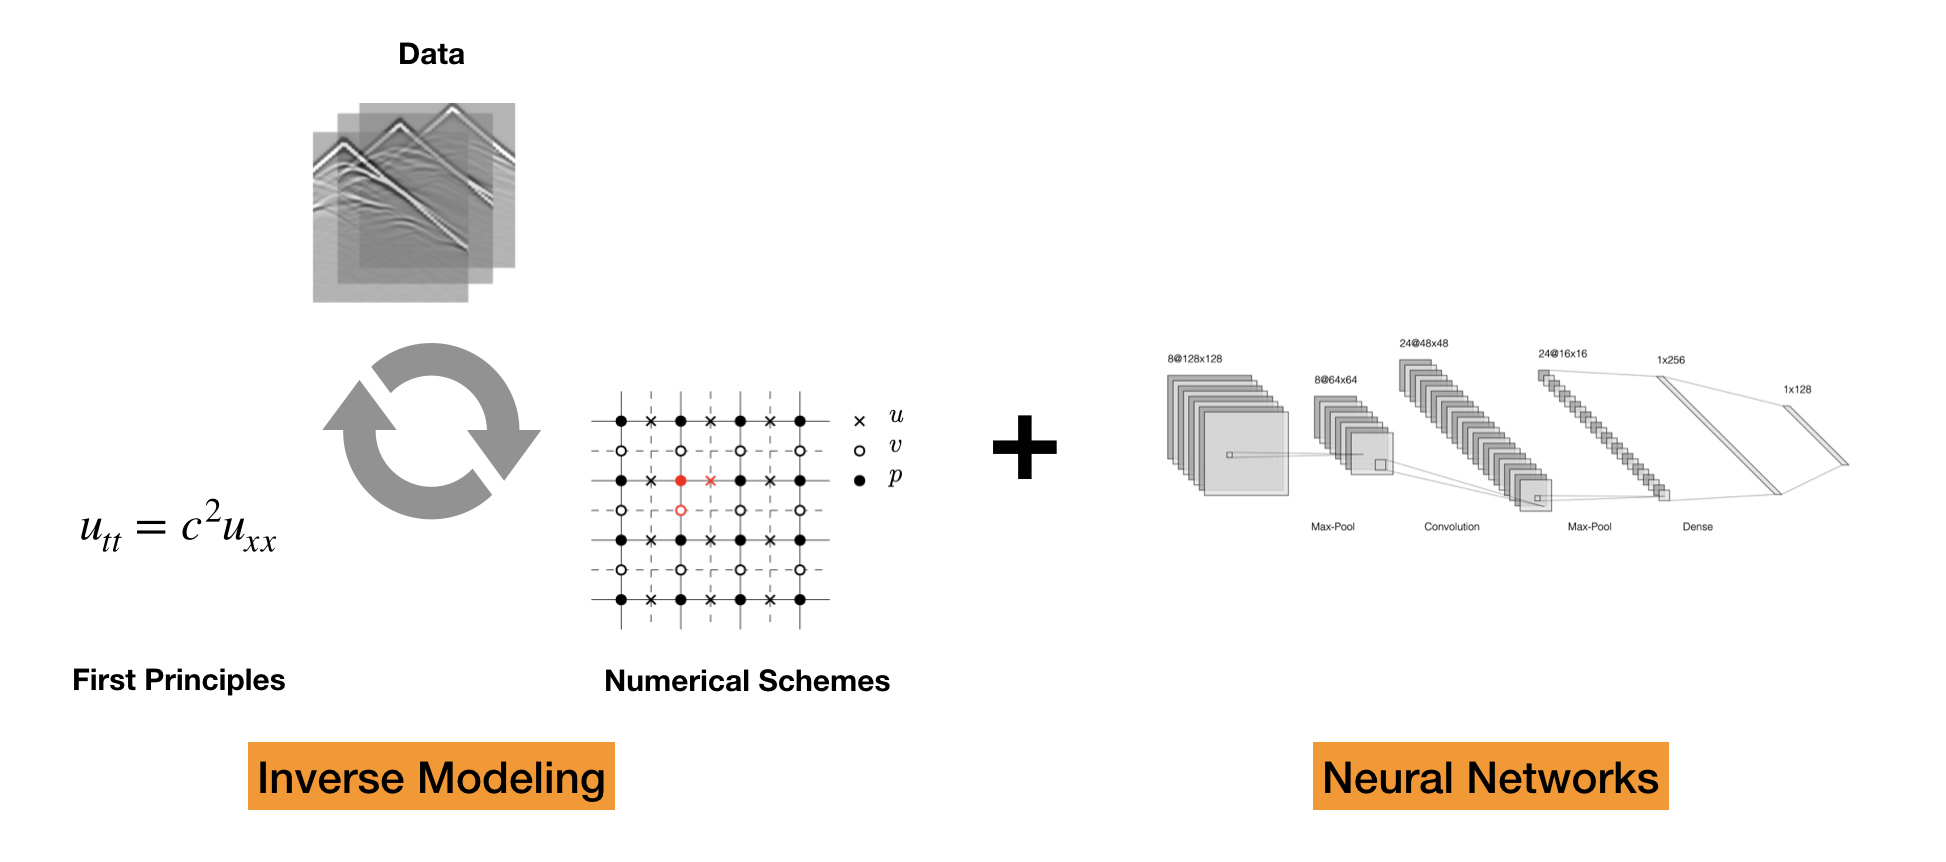
\includegraphics[width=0.75\textwidth]{figures/physics_based_machine_learning.png}
\end{figure}
\end{frame}


\section{Methodology}


\begin{frame}
	\frametitle{Gradient Based Optimization}
	\begin{equation}\label{equ:opt}
	\min_{\theta} L_h(u_h) \quad \mathrm{s.t.}\; F_h(\theta, u_h) = 0
	\end{equation}
	
	\begin{itemize}
		\item We can now apply a gradient-based optimization method to (\ref{equ:opt}).
		\item The key is to \textcolor{red}{calculate the gradient descent direction} $g^k$
		$$\theta^{k+1} \gets \theta^k - \alpha g^k$$ 
	\end{itemize}
	
	\begin{figure}[hbt]
		\centering
		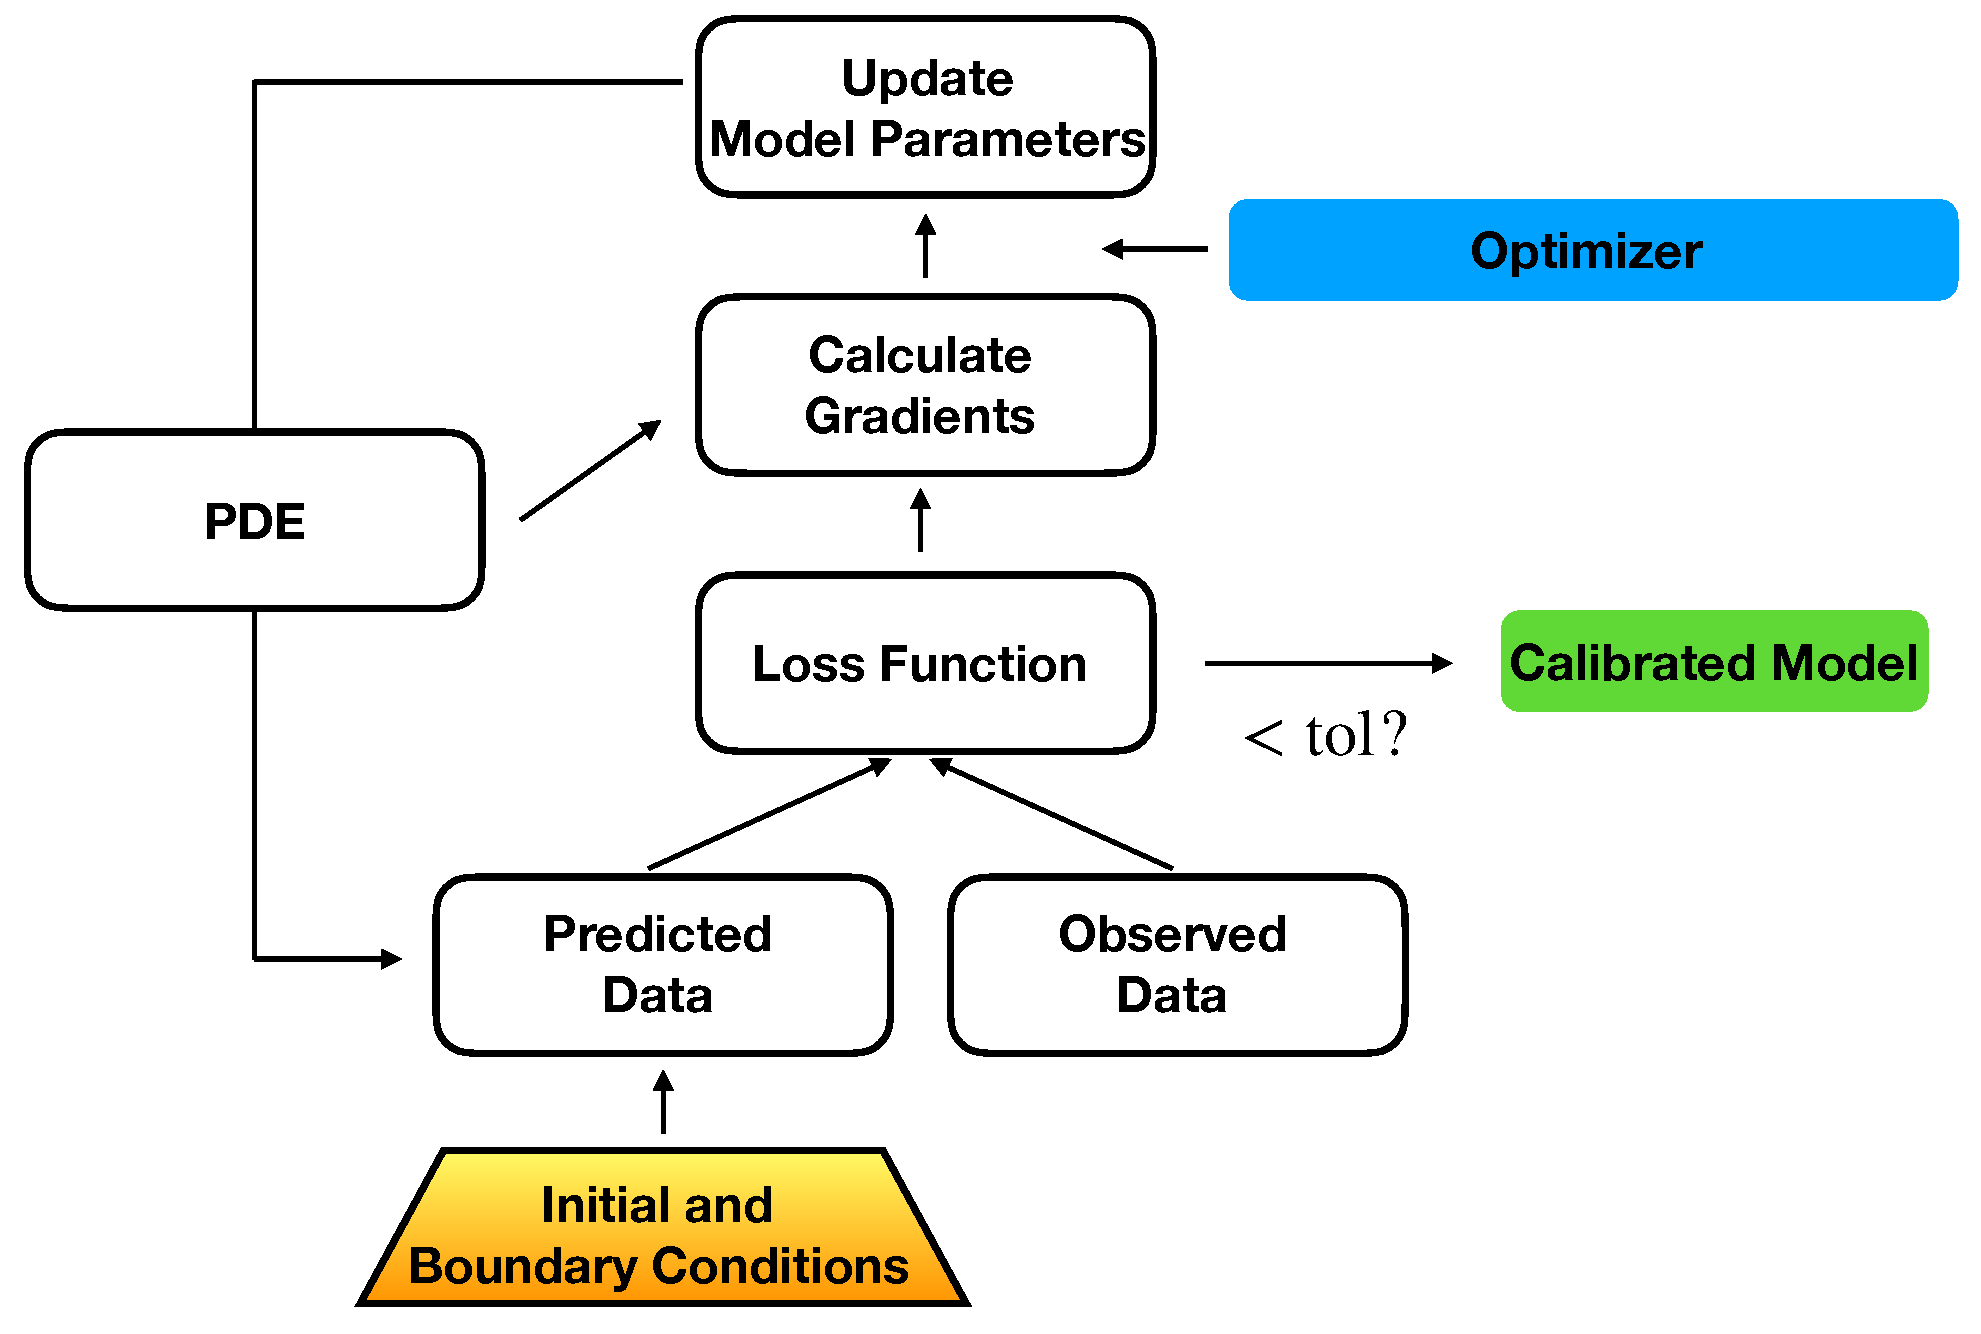
\includegraphics[width=0.6\textwidth]{figures/im.pdf}
	\end{figure}
	
\end{frame}




\begin{frame}
	
	
	\frametitle{Challenges in AD}
	
	
	\begin{minipage}[t]{0.49\textwidth}
		\vspace{-3cm}
		\begin{itemize}
			\item Most AD frameworks only deal with explicit operators, i.e., the functions that has analytical derivatives, or composition of these functions. 
			\item Many scientific computing algorithms are \textcolor{red}{iterative} or \textcolor{red}{implicit} in nature $\Rightarrow$ Physics Constrained Learning (PCL)
		\end{itemize}
	\end{minipage}~
	\begin{minipage}[t]{0.49\textwidth}
		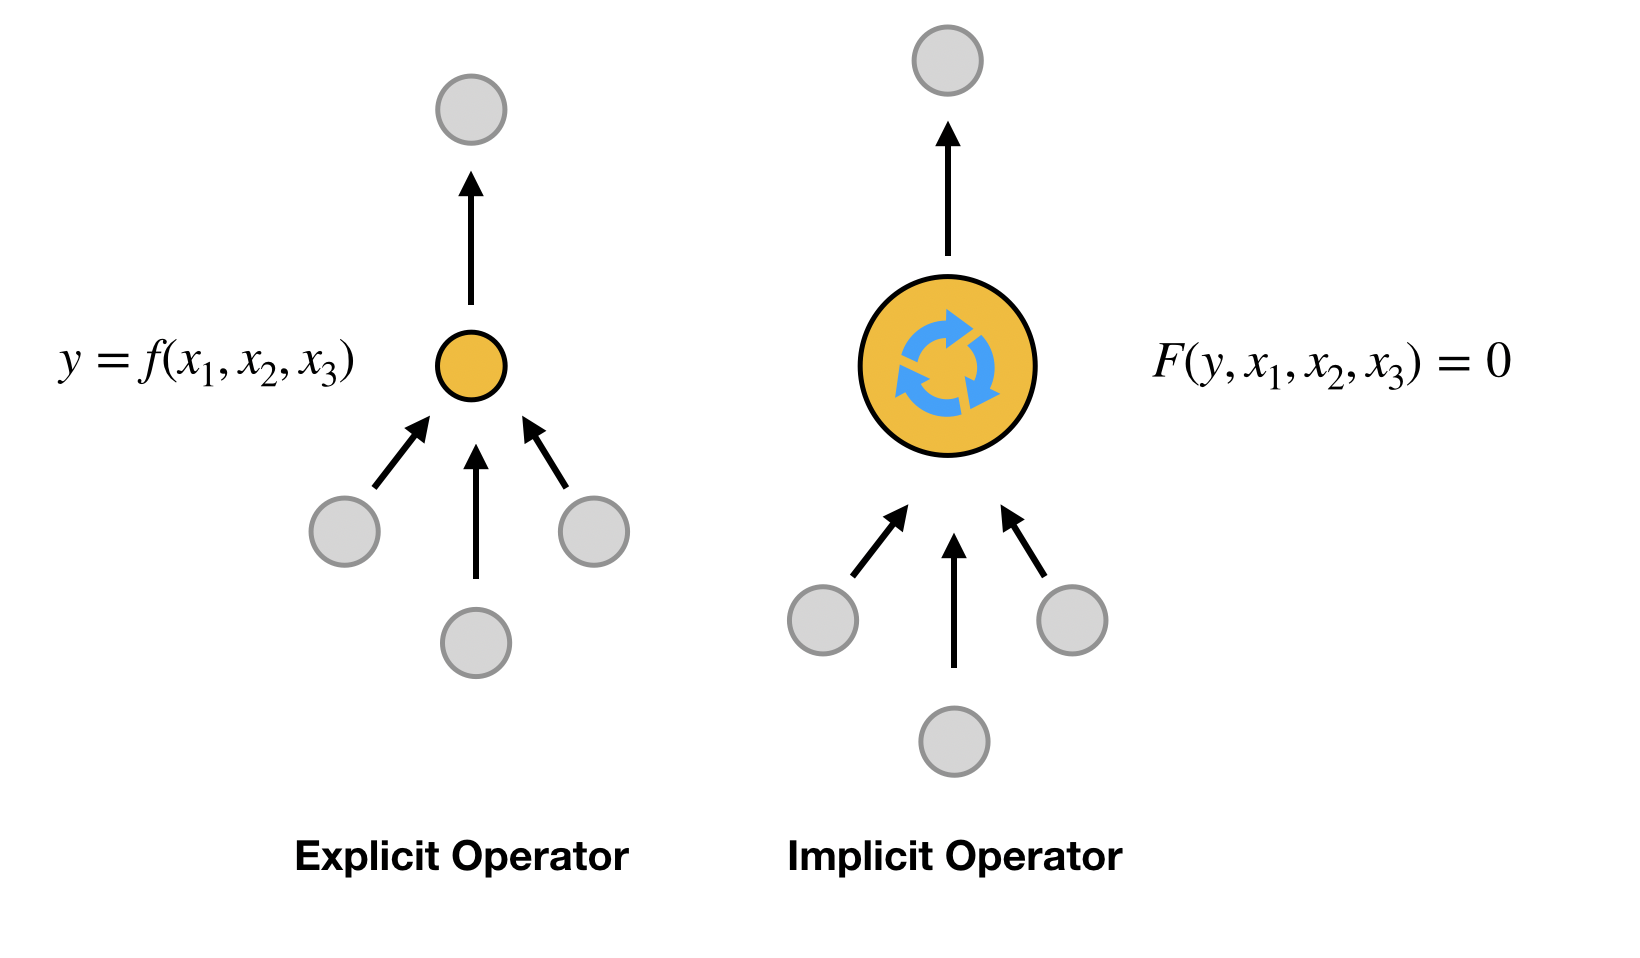
\includegraphics[width=1.0\textwidth]{figures/sim.png}
	\end{minipage}
	
	% Please add the following required packages to your document preamble:
	% \usepackage{booktabs}
	\begin{table}[]
		\begin{tabular}{@{}lll@{}}
			\toprule
			Linear/Nonlinear & Explicit/Implicit & Expression   \\ \midrule
			Linear           & Explicit          & $y=Ax$       \\
			Nonlinear        & Explicit          & $y = F(x)$   \\
			\textbf{Linear}           & \textbf{Implicit}          & $Ay = x$     \\
			\textbf{Nonlinear}        & \textbf{Implicit}          & $F(x,y) = 0$ \\ \bottomrule
		\end{tabular}
	\end{table}
\end{frame}


\begin{frame}
	\frametitle{Example}
	
	\begin{itemize}
		\item Consider a function $f:x\rightarrow y$, which is implicitly defined by 
		$$F(x,y) = x^3 - (y^3+y) = 0$$
		If not using the cubic formula for finding the roots, the forward computation consists of iterative algorithms, such as the Newton's method and bisection method
	\end{itemize}
	
	
	
	\begin{minipage}[t]{0.48\textwidth}
		\centering
		\begin{algorithmic}
			\State $y^0 \gets 0$
			\State $k \gets 0$
			\While {$|F(x, y^k)|>\epsilon$}
			\State $\delta^k \gets F(x, y^k)/F'_y(x,y^k)$
			\State $y^{k+1}\gets y^k - \delta^k$
			\State $k \gets k+1$
			\EndWhile
			\State \textbf{Return} $y^k$
		\end{algorithmic}
	\end{minipage}~
	\begin{minipage}[t]{0.48\textwidth}
		\centering
		\begin{algorithmic}
			\State $l \gets -M$, $r\gets M$, $m\gets 0$
			\While {$|F(x, m)|>\epsilon$}
			\State $c \gets \frac{a+b}{2}$
			\If{$F(x, m)>0$}
			\State $a\gets m$
			\Else
			\State $b\gets m$
			\EndIf
			\EndWhile
			\State \textbf{Return} $c$
		\end{algorithmic}
		
	\end{minipage}	
	
\end{frame}

\begin{frame}
	\frametitle{Example}
	
	\begin{itemize}
		%		\item A simple approach is to save part or all intermediate steps, and ``back-propagate''. This approach is expensive in both computation and memory\footnote{Ablin, Pierre, Gabriel Peyrᅵ, and Thomas Moreau. ``Super-efficiency of automatic differentiation for functions defined as a minimum.''}.
		%		\item Nevertheless, the simple approach works in some scenarios where accuracy or cost is not an issue, e.g., automatic differetiation of soft-DTW and Sinkhorn distance. 
		\item An efficient way to do automatic differentiation is to apply the \textcolor{red}{implicit function theorem}. For our example, $F(x,y)=x^3-(y^3+y)=0$; treat $y$ as a function of $x$ and take the derivative on both sides
		$$3x^2 - 3y(x)^2y'(x)-y'(x)=0\Rightarrow y'(x) = \frac{3x^2}{3y^2+1}$$
		The above gradient is \textcolor{red}{exact}.
	\end{itemize}
	\begin{center}
		\textbf{Can we apply the same idea to inverse modeling?}
	\end{center}
	
\end{frame}



\begin{frame}
	\frametitle{Physics Constrained Learning}
	$${\small    \min_{\theta}\; L_h(u_h) \quad \mathrm{s.t.}\;\; F_h(\theta, u_h) = 0}$$
	\begin{itemize}
		\item Assume that we solve for $u_h=G_h(\theta)$ with $F_h(\theta, u_h)=0$, and then
		$${\small\tilde L_h(\theta)  = L_h(G_h(\theta))}$$
		\item Applying the \textcolor{red}{implicit function theorem}
		{  \scriptsize
			\begin{equation*}
			\frac{{\partial {F_h(\theta, u_h)}}}{{\partial \theta }} + {\frac{{\partial {F_h(\theta, u_h)}}}{{\partial {u_h}}}}
			\textcolor{red}{\frac{\partial G_h(\theta)}{\partial \theta}}
			= 0 \Rightarrow
			\textcolor{red}{\frac{\partial G_h(\theta)}{\partial \theta}} =  -\Big( \frac{{\partial {F_h(\theta, u_h)}}}{{\partial {u_h}}} \Big)^{ - 1} \frac{{\partial {F_h(\theta, u_h)}}}{{\partial \theta }}
			\end{equation*}
		}
		\item Finally we have
		{\scriptsize
			\begin{equation*}
			\boxed{\frac{{\partial {{\tilde L}_h}(\theta )}}{{\partial \theta }}
				= \frac{\partial {{ L}_h}(u_h )}{\partial u_h}\frac{\partial G_h(\theta)}{\partial \theta}=
				- \textcolor{red}{ \frac{{\partial {L_h}({u_h})}}{{\partial {u_h}}} } \;
				\textcolor{blue}{ \Big( {\frac{{\partial {F_h(\theta, u_h)}}}{{\partial {u_h}}}\Big|_{u_h = {G_h}(\theta )}} \Big)^{ - 1} } \;
				\textcolor{ForestGreen}{ \frac{{\partial {F_h(\theta, u_h)}}}{{\partial \theta }}\Big|_{u_h = {G_h}(\theta )} }
			}
			\end{equation*}
		}
		
	\end{itemize}
	
\end{frame}




\begin{frame}
	\frametitle{Scientific Machine Learning Inverse Modeling Toolkit}

	
		\begin{figure}[hbt]
		\centering
  \includegraphics[width=0.6\textwidth]{figures/adcme_logo}
\end{figure}

\begin{minipage}[t]{0.33\textwidth}
	\begin{center}
\textcolor{teal}{\textbf{High Performance}}		
	\end{center}

	
	Solves large-scale problems with TensorFlow backend and MPI-based distributed optimization for scientific computing. 
\end{minipage}~
\begin{minipage}[t]{0.33\textwidth}

\begin{center}
\textcolor{red}{\textbf{Easy to Use}}
	\end{center}

Provides high-level syntax, which is compatible with Julia syntax, for implementing numerical schemes. 
\end{minipage}~
\begin{minipage}[t]{0.33\textwidth}

\begin{center}
\textcolor{violet}{Broad Applicability}
	\end{center}
	
	
Constructs multiple physical models using toolkits from ADCME ecosystem and extends capabilities by custom operators. 
\end{minipage}
\end{frame}
\vspace{-1.0cm}

\begin{frame}
	\frametitle{ADCME Architecture}
	
	\begin{figure}[hbt]
		\centering
  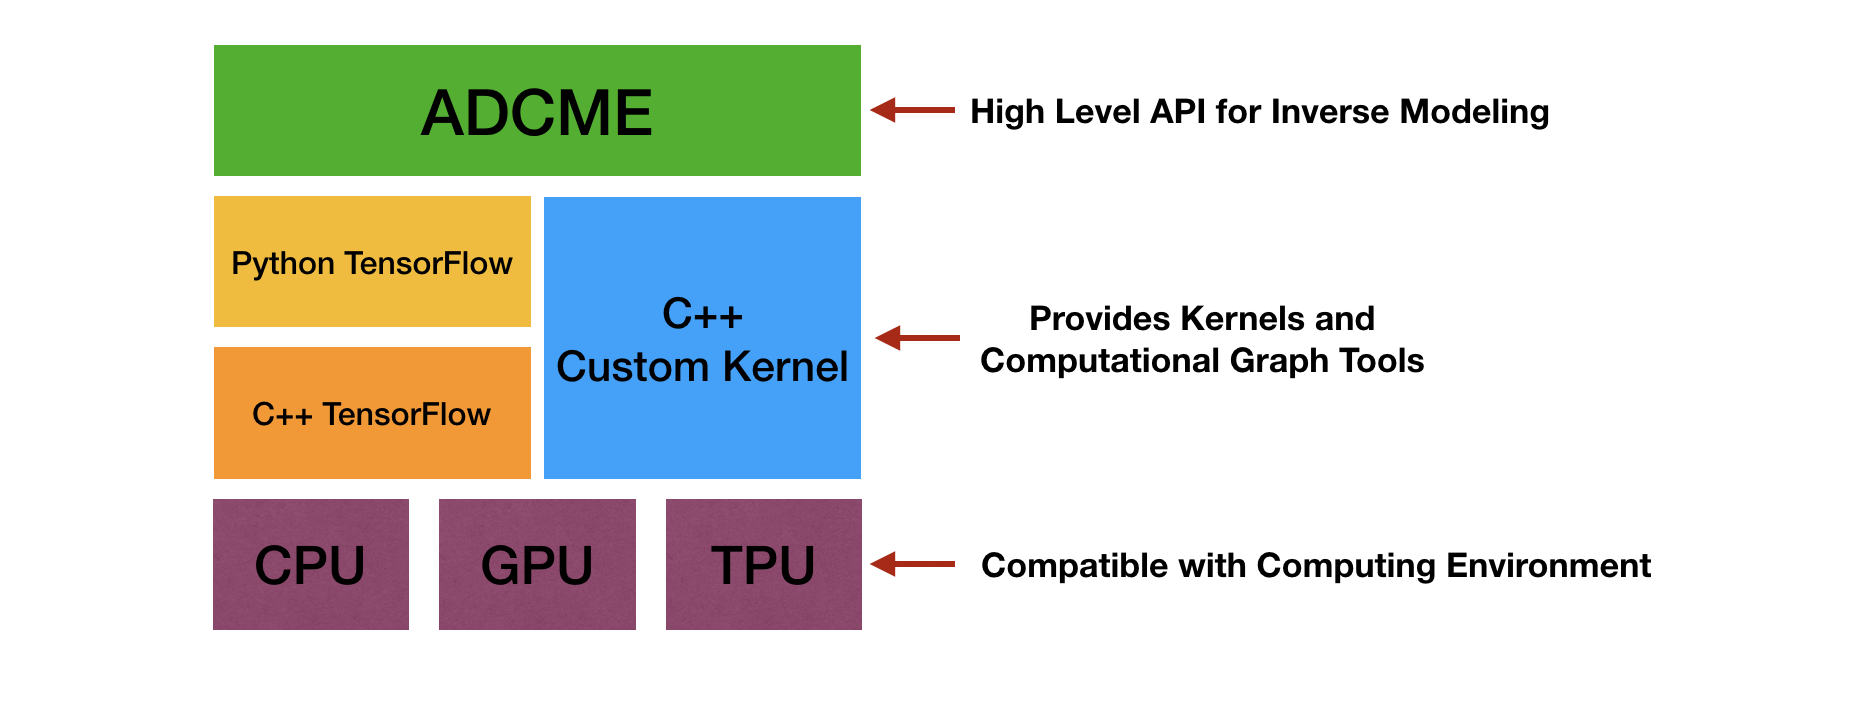
\includegraphics[width=1.0\textwidth]{figures/kernel}
\end{figure}
\vspace{-1.0cm}
Targeting at \textcolor{red}{scientific computing}: 
\begin{itemize}
	\item Sparse linear algebra;
	\item MPI-based distributed computing;
	\item Domain specific numerical schemes: seismic inversion (ADSeismic.jl), fluid dynamics (FwiFlow.jl), geomechanics (AdFem.jl), solid mechanics (NNFEM.jl), $\ldots$
\end{itemize}
\end{frame}

\begin{frame}
	\frametitle{Distributed Optimization}
	\begin{itemize}
		\item ADCME also supports MPI-based distributed computing. The parallel model is designed specially for scientific computing. 
	\end{itemize}
	\begin{figure}[hbt]
		\centering
  \includegraphics[width=0.49\textwidth]{figures/distributed1}~
  \includegraphics[width=0.49\textwidth]{figures/distributed2}
\end{figure}
\end{frame}

\begin{frame}
	\frametitle{Estimating Coefficients from Data using ADCME}
	
	\begin{align*}
		-\textcolor{red}{b} u''(x) + u(x) &= f(x), \quad x\in [0,1], \quad u(0) = u(1) = 0\\ 
		f(x) &= 8+4x-4x^2
	\end{align*}
	
	
	\begin{itemize}
		\item Data: $u(0.5)=1$
		\item Finite difference:
		\begin{align*}
			-\textcolor{red}{b}\frac{u_{i+1} + u_{i-1} - 2u_i}{h^2} + u_i &= f(x_i)\\
			\mathbf{B} \mathbf{u} &= \mathbf{f}
		\end{align*}
		\begin{enumerate}
			\item Compute $u_i$ as a function of $b$;
			\item Minimize $(u_k - u(0.5))^2$, here $x_k = 0.5$.
		\end{enumerate}
	\end{itemize}
	
\end{frame}

\begin{frame}[fragile]
	\frametitle{Estimating Coefficients from Data using ADCME}
	\vspace{-0.3cm}
	{\small
	\begin{lstlisting}
using LinearAlgebra
using ADCME

n = 101 # number of grid nodes in [0,1]
h = 1/(n-1)
x = LinRange(0,1,n)[2:end-1]

b = Variable(10.0) 
A = diagm(0=>2/h^2*ones(n-2), 
          -1=>-1/h^2*ones(n-3), 1=>-1/h^2*ones(n-3)) 
B = b*A + I  # I stands for the identity matrix
f = @. 4*(2 + x - x^2) 
u = B\f # solve the equation using built-in linear solver
ue = u[div(n+1,2)] # extract values at x=0.5
loss = (ue-1.0)^2 

# Optimization
sess = Session(); init(sess) 
BFGS!(sess, loss)

println("Estimated b = ", run(sess, b))
	\end{lstlisting}
	}
\end{frame}

\begin{frame}[fragile]
	\frametitle{Domain Specific Numerical Schemes}
	
	\begin{equation*}
		-\nabla \cdot (\textcolor{red}{\kappa} \nabla u) = f, \qquad u|_{\partial \Omega} = 0 
	\end{equation*}
	
	\begin{itemize}
		\item Weak form 
		\begin{equation*}
			\int_\Omega \kappa \nabla u \cdot \nabla v d\mathbf{x} = \int_\Omega f v d\mathbf{x}
		\end{equation*}
		\item The variational problem is transcribed into numerical simulation using domain specific implementations from AdFem.jl:
	\end{itemize}
	{\small
	\begin{lstlisting}
A = constant(compute_fem_laplace_matrix1(kappa, m, n, h))
F = eval_f_on_gauss_pts(f, m, n, h)
bd = bcnode("all", m, n, h)
A, _ = fem_impose_Dirichlet_boundary_condition1(A, bd, 
                                                m, n, h)
rhs = compute_fem_source_term1(F, m, n, h)
rhs[bd] .= 0.0
sol = A\rhs\end{lstlisting}
}
\end{frame}



\begin{frame}
	\frametitle{A General Approach to Inverse Modeling}
	\begin{figure}[hbt]
  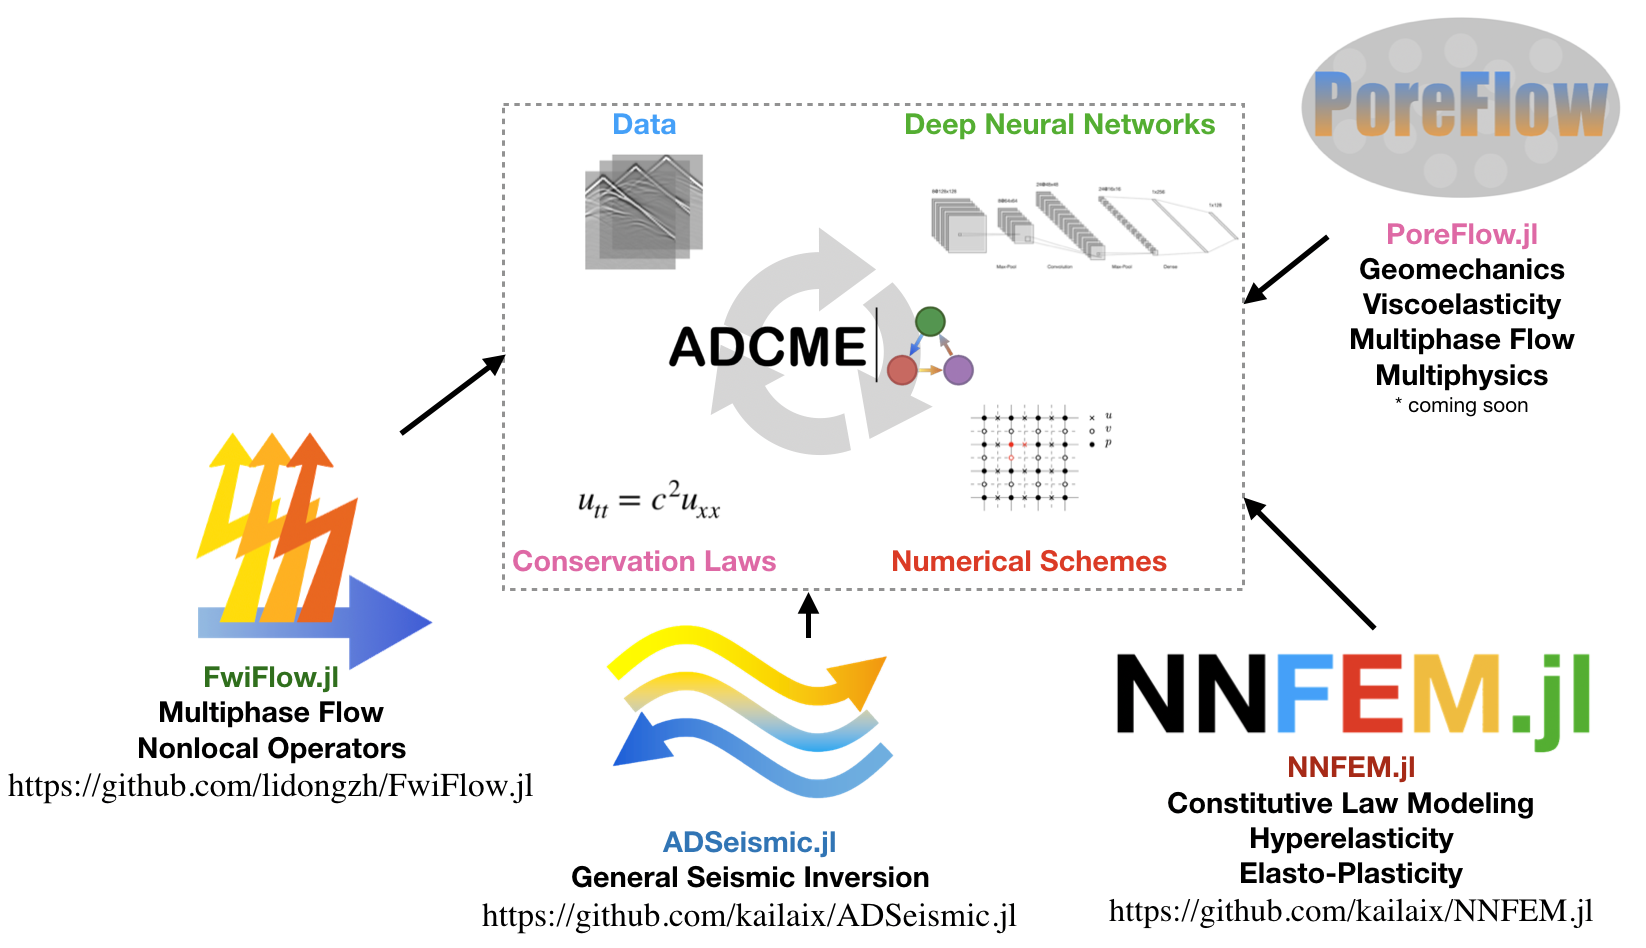
\includegraphics[width=1.0\textwidth]{figures/summary.png}
\end{figure}

\end{frame}


\section{Applications}



\begin{frame}
	\frametitle{ADSeismic.jl: A General Approach to Seismic Inversion}
	\begin{itemize}
		\item Many seismic inversion problems can be solved within a unified framework. 
	\end{itemize}
	\begin{figure}[hbt]
  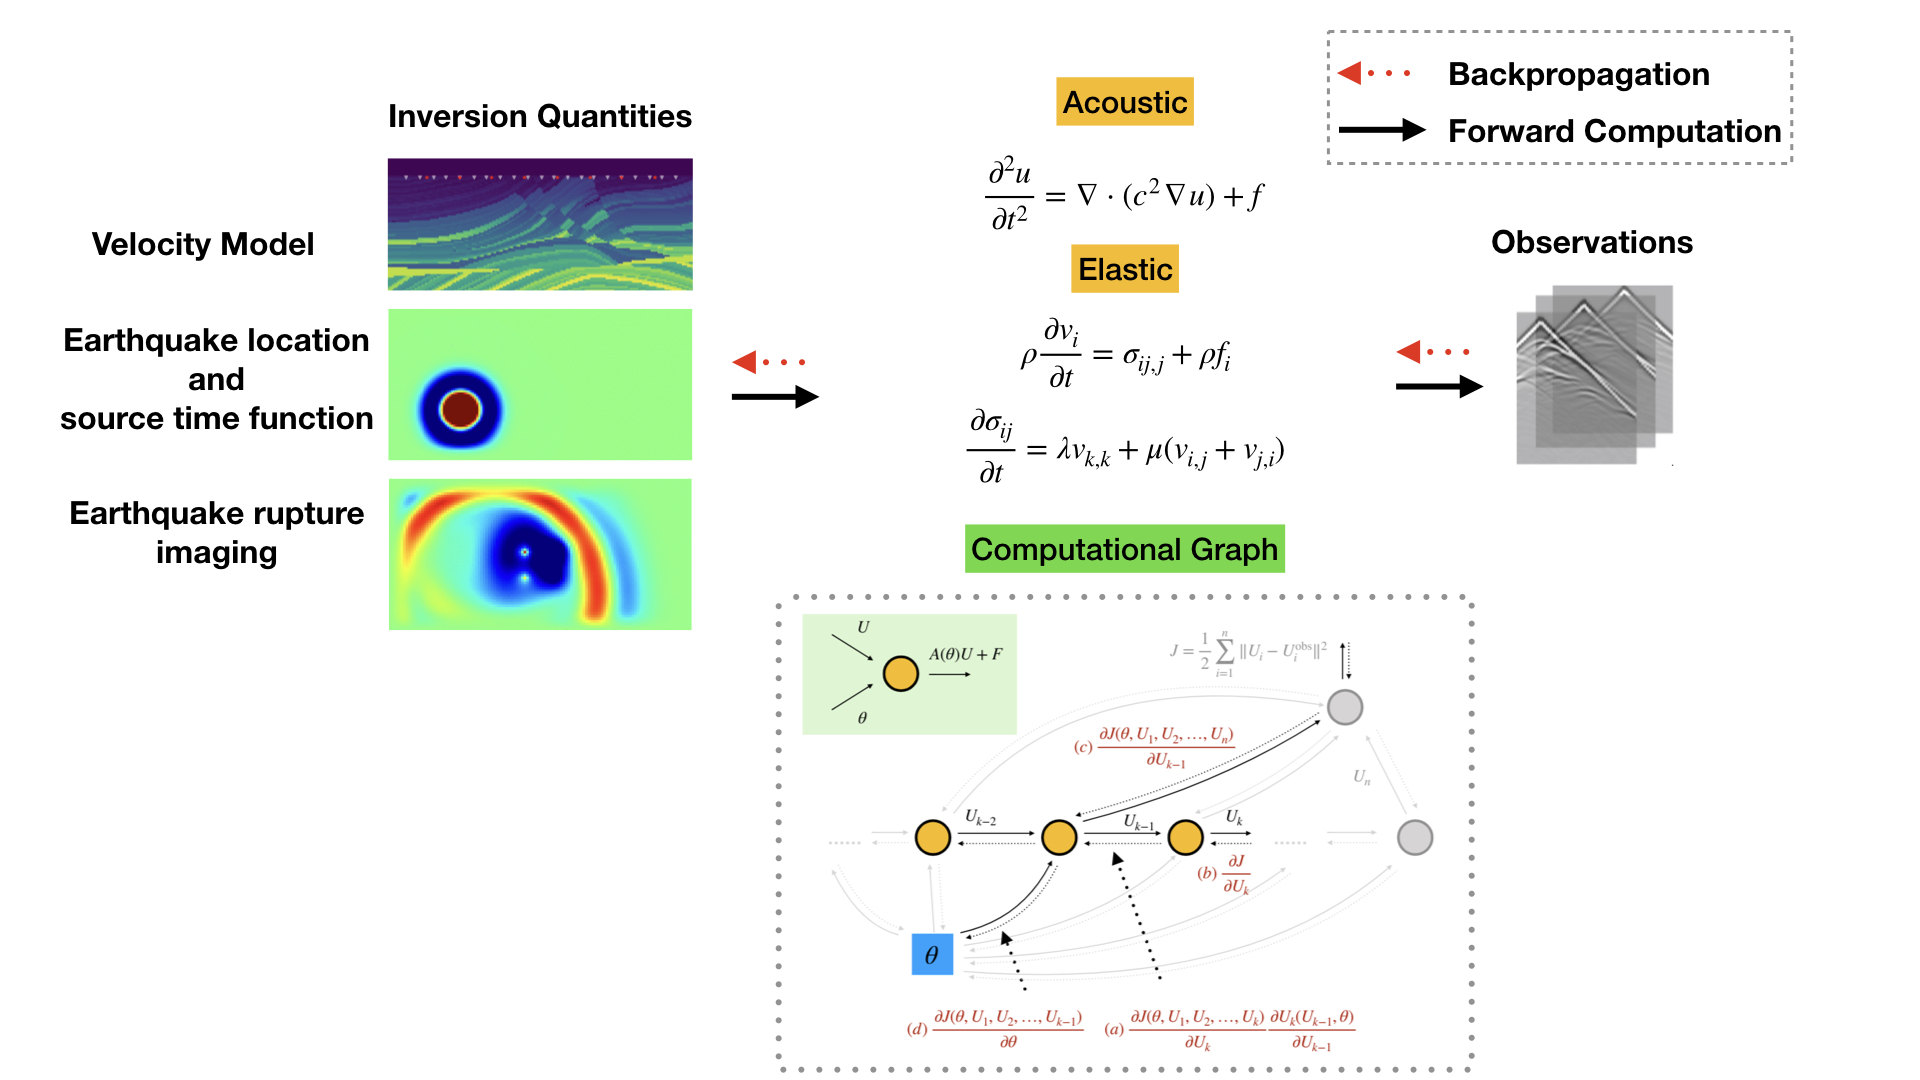
\includegraphics[width=1.0\textwidth]{figures/adseimic.jpeg}
\end{figure}
	
\end{frame}

\begin{frame}
	\frametitle{ADSeismic.jl: Earthquake Location Example}
	\begin{itemize}
		\item The earthquake source function is parameterized by ($g(t)$ and $x_0$ are unknowns)
		$$f(x, t) =  \frac{g(t)}{2\pi \sigma^2} \exp \left( -\frac{||x - x_0||^2}{2 \sigma^2} \right)$$
	\end{itemize}
	\begin{figure}[hbt]
  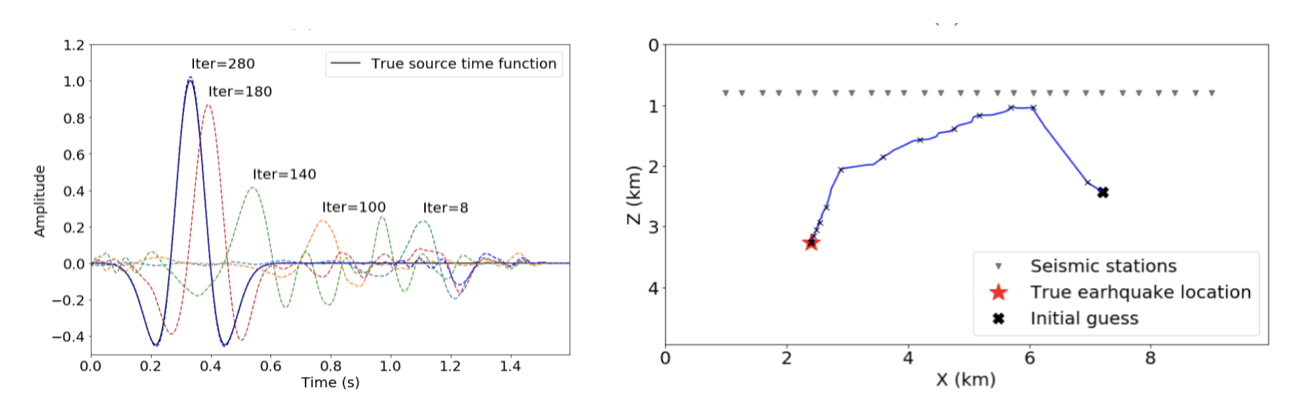
\includegraphics[width=1.0\textwidth]{figures/source_time}
\end{figure}
\end{frame}


\begin{frame}
	\frametitle{ADSeismic.jl: Benchmark}
	\begin{itemize}
		\item ADCME makes the heterogeneous computation capability of TensorFlow available for scientific computing. 
	\end{itemize}
	\begin{figure}[hbt]
  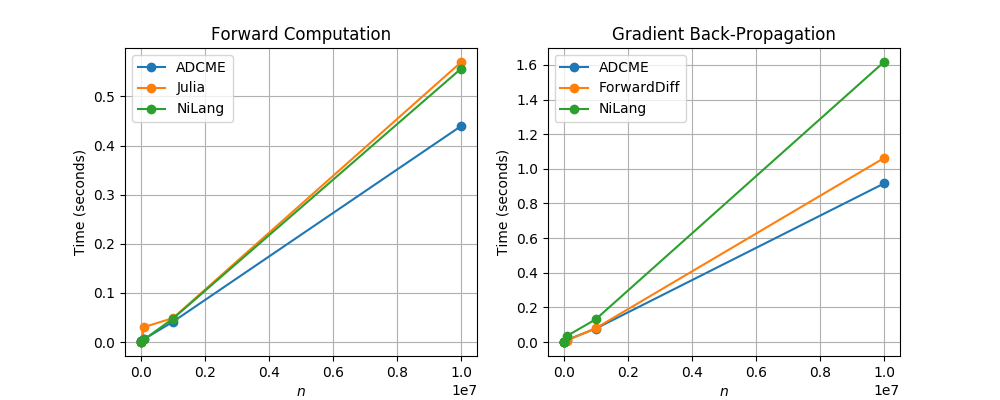
\includegraphics[width=0.7\textwidth]{figures/benchmark}
\end{figure}
\end{frame}

\begin{frame}
	\frametitle{NNFWI: Neural-network-based Full-Waveform Inversion}
	
	\begin{itemize}
		\item Estimate velocity models from seismic observations. 
	\end{itemize}
	\begin{minipage}[t]{0.3\textwidth}
		\begin{equation*}
\qquad\frac{\partial^2 u}{\partial t^2} = \nabla \cdot (\textcolor{red}{m}^2 \nabla u) + f
\end{equation*}
	\end{minipage}~
	\begin{minipage}[t]{0.69\textwidth}
	\begin{figure}[hbt]
	\centering
  \includegraphics[width=0.7\textwidth]{figures/bp}
\end{figure}
\end{minipage}
	


\begin{figure}[hbt]
  \includegraphics[width=0.6\textwidth]{figures/fwi}
\end{figure}
\end{frame}

\begin{frame}
	\frametitle{NNFWI: Neural-network-based Full-Waveform Inversion}

\begin{itemize}
	\item Inversion results with a noise level $\sigma = \sigma_0$
	\begin{figure}[hbt]
	\centering
  \includegraphics[width=0.8\textwidth]{figures/bp_results}
\end{figure}

\item Inversion results for the same loss function value:
\begin{figure}[hbt]
\centering
  \includegraphics[width=0.8\textwidth]{figures/bp_results_2}
\end{figure}

\end{itemize}

\end{frame}

\begin{frame}
	\frametitle{Constitutive Modeling}
	
	\begin{figure}[hbt]
\centering
  \includegraphics[width=1.0\textwidth]{figures/ad_constitutive_modeling}
\end{figure}
\end{frame}


\begin{frame}
	\frametitle{NNFEM.jl: Constitutive Modeling}
	
	\begin{equation}\label{equ:momentum}
  \begin{aligned}
		\underbrace{\sigma_{ij,j}}_{\mbox{stress}} + \rho \underbrace{b_i}_{\mbox{external force}} &= \rho \underbrace{\ddot u_i}_{\mbox{velocity}}\\
		\underbrace{\varepsilon_{ij}}_{\mbox{strain}} &= \frac{1}{2}(u_{j,i}+u_{i,j})
	\end{aligned}
\end{equation}

	
	\begin{itemize}
		\item \textbf{Observable}: external/body force $b_i$, displacements $u_i$ (strains $\varepsilon_{ij}$ can be computed from $u_i$); density $\rho$ is known.  
		\item \textbf{Unobservable}: stress $\sigma_{ij}$. 
		\item Data-driven Constitutive Relations: modeling the strain-stress relation using a neural network
\begin{equation}\label{equ:nn}
  	\boxed{\mbox{stress} =\mathcal{M}_{\theta}(\mbox{strain},\ldots)}
\end{equation}
		and the neural network is trained by coupling (1) and (2).
	\end{itemize}


\end{frame}

\begin{frame}
	\frametitle{NNFEM.jl: Robust Constitutive Modeling}
	\begin{itemize}
\item Proper form of constitutive relation is crucial for numerical stability
{\footnotesize\begin{align*}
 \mbox{Elasticity} &\Rightarrow \bm\sigma = \mathsf{C}_{\theta}\bm\epsilon \\
\mbox{Hyperelasticity } &\Rightarrow \begin{cases}\bm\sigma =\mathcal{M}_{\theta}(\bm\epsilon) & \mbox{(Static)} \\
\bm{\sigma}^{n+1}  =  \ChoL_{\bt}(\bm\epsilon^{n+1}) \ChoL_{\bt}(\bm\epsilon^{n+1})^T (\bm{\epsilon}^{n+1} - \bm{\epsilon}^{n})  + \bm{\sigma}^{n}  & \mbox{(Dynamic)} \end{cases} \\
	\mbox{Elaso-Plasticity} &\Rightarrow \bm\sigma^{n+1} = \ChoL_{\bt}(\bm\epsilon^{n+1},\bm{\epsilon}^{n},\bm{\sigma}^{n}) \ChoL_{\bt}(\bm\epsilon^{n+1},\bm{\epsilon}^{n},\bm{\sigma}^{n})^T (\bm{\epsilon}^{n+1} - \bm{\epsilon}^{n})  + \bm{\sigma}^{n} 
\end{align*}
}{\footnotesize$$\ChoL_{\bt} = \begin{bmatrix}
L_{1111}  &  & &  &       &\\
L_{2211}  & L_{2222} & &   & &\\
 L_{3311}  &  L_{3322}               & L_{3333} &  & &\\
               &                 &                 & L_{2323}&  &\\
              &               &                  &                & L_{1313} &\\
              &                 &                  &                &                 &L_{1212}\\
\end{bmatrix}$$}
	\item \textcolor{red}{Weak convexity}: $\ChoL_{\bt}\ChoL_{\bt}^T \succ 0$
	\item \textcolor{red}{Time consistency}:  $\bm\sigma^{n+1} \rightarrow \bm \sigma^n$ when $\bm\epsilon^{n+1} \rightarrow \bm \epsilon^n$
\end{itemize}

\end{frame}

\begin{frame}
	\frametitle{NNFEM.jl: Robust Constitutive Modeling}
	\begin{itemize}
	 \item Weak form of balance equations of linear momentum 
	{\footnotesize
	\begin{align*}
		P_i(\theta) &= \int_V \rho \ddot u_i \delta u_i dVt + \int_{V} \textcolor{blue}{\underbrace{\textcolor{blue}{\sigma_{ij}(\theta)}}_{\mathclap{\textcolor{blue}{\mbox{embedded neural network}}}}} \delta \varepsilon_{ij}dV\\
		F_i &= \int_{V}\rho b_i \delta u_i dV + \int_{\partial V} t_i\delta u_idS
	\end{align*}
	}
	\item Train the neural network by 
	{\scriptsize $$\boxed{L(\theta) = \min_{\theta}\;\sum_{i=1}^N(P_i(\theta) - F_i)^2}$$}
	The gradient $\nabla L(\theta)$ is computed via automatic differentiation.
	\end{itemize}
	\begin{figure}[hbt]
  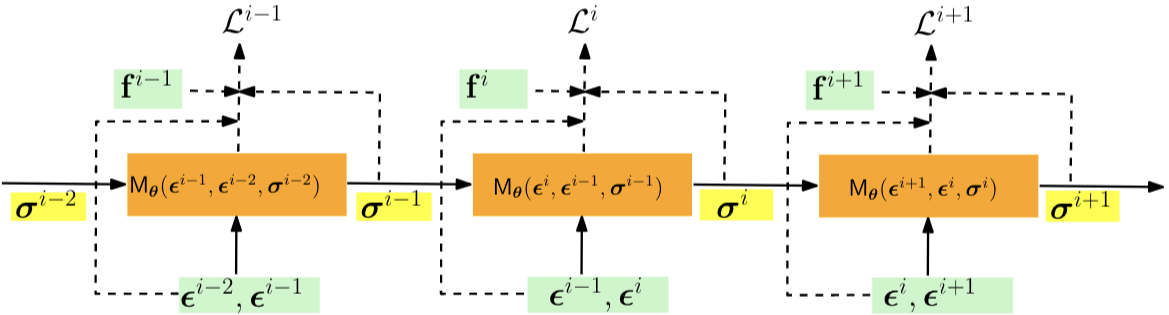
\includegraphics[width=0.75\textwidth]{figures/rnn}
\end{figure}

\end{frame}

\begin{frame}
	\frametitle{NNFEM.jl: Robust Constitutive Modeling}
\begin{figure}[hbt]
  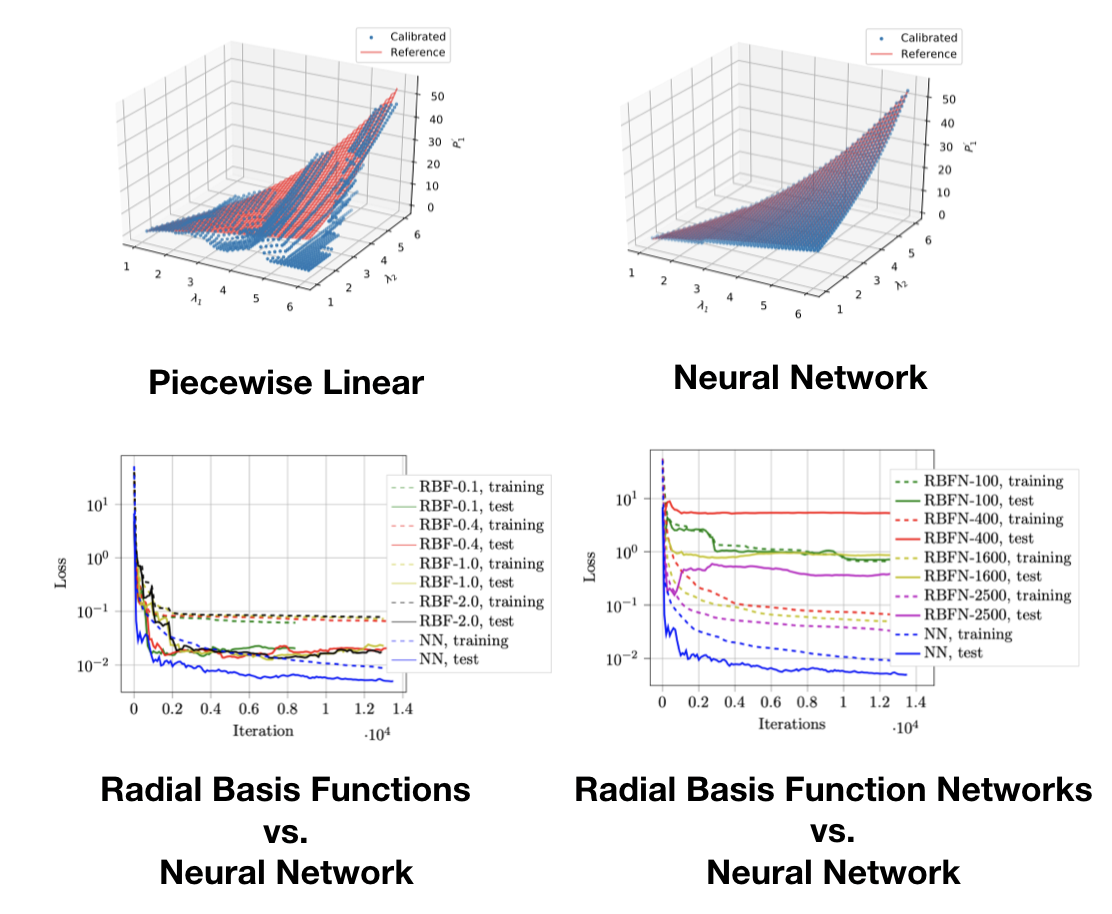
\includegraphics[width=0.8\textwidth]{figures/vs}
\end{figure}
\end{frame}


\begin{frame}
	\frametitle{NNFEM.jl: Robust Constitutive Modeling}
	\begin{itemize}
		\item Comparison of different neural network architectures 
		\begin{align*}
			\bm\sigma^{n+1} &= \ChoL_{\bt}(\bm\epsilon^{n+1},\bm{\epsilon}^{n},\bm{\sigma}^{n}) \ChoL_{\bt}(\bm\epsilon^{n+1},\bm{\epsilon}^{n},\bm{\sigma}^{n})^T (\bm{\epsilon}^{n+1} - \bm{\epsilon}^{n})  + \bm{\sigma}^{n} \\
			\bm{\sigma}^{n+1} &=  \mathsf{NN}_{\bt}(\bm\epsilon^{n+1},\bm{\epsilon}^{n},\bm{\sigma}^{n})\\
			\bm{\sigma}^{n+1} &=  \mathsf{NN}_{\bt}(\bm\epsilon^{n+1},\bm{\epsilon}^{n},\bm{\sigma}^{n}) + \bm{\sigma}^{n}
		\end{align*}
	\end{itemize}
\begin{figure}[hbt]
  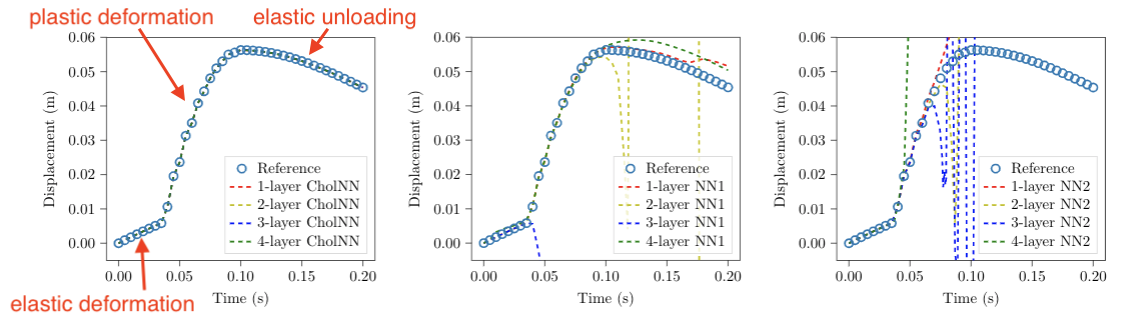
\includegraphics[width=1.0\textwidth]{figures/nncons}
\end{figure}
\end{frame}



\begin{frame}
	\frametitle{AdFem.jl: FEM/FVM on Structured Grids}
	\begin{itemize}
		\item Steady-state Navier-Stokes equation
		\begin{equation*}
	\begin{aligned}
		(\mathbf{u} \cdot \nabla) \mathbf{u} &=
    -\frac{1}{\rho} \nabla p + \nabla\cdot (\textcolor{red}{\nu} \nabla \mathbf{u}) + \mathbf{g}\\
\nabla \cdot \mathbf{u} &= 0
	\end{aligned}
    \end{equation*}
    
    \item Inverse problem are ubiquitous in fluid dynamics:
    
    \begin{figure}[hbt]
    \centering
  \includegraphics[width=0.4\textwidth]{figures/icepack}~
  \includegraphics[width=0.4\textwidth]{figures/covid}
  \caption{Left: electronic cooling; right: nasal drug delivery.}
\end{figure}

	\end{itemize}
	    
  \end{frame}
  
  
  \begin{frame}
  	\frametitle{AdFem.jl: FEM/FVM on Structure Grids}
  	
  	\begin{figure}[hbt]
    \centering
  \includegraphics[width=0.49\textwidth]{figures/advertisement}~
  \includegraphics[width=0.49\textwidth]{figures/computational_graph}
\end{figure}
  \end{frame}

  
  
  \begin{frame}
  	\frametitle{AdFem.jl: FEM/FVM on Structure Grids}
\begin{itemize}
	\item Data: $(u, v)$
	\item Unknown: $\nu(\mathbf{x})$ (represented by a deep neural network)
	\item Prediction: $p$ (absent in the training data) 
	\item The DNN provides regularization, which generalizes the estimation better!
	\end{itemize}
  	\begin{figure}[hbt]
    \centering
  \includegraphics[width=1.0\textwidth]{figures/ns_result}~
\end{figure}
  \end{frame}



\section{Some Perspectives}

\begin{frame}
	\frametitle{A Parameter/Function Learning View of Inverse Modeling}
	% Please add the following required packages to your document preamble:
% \usepackage{booktabs}
\begin{itemize}
	\item Most inverse modeling problems can be classified into 4 categories. To be more concrete, consider the PDE for describing physics
	\begin{equation}
		\nabla \cdot (\textcolor{red}{\theta} \nabla u(x)) = 0\quad \mathcal{B}\mathcal{C}(u(x)) = 0
	\end{equation}
	We observe some quantities depending on the solution $u$ and want to estimate $\theta$.
\end{itemize}
{
\tiny
\begin{table}[]
\begin{tabular}{@{}lllc@{}}
\toprule
Expression                                       & Description                & ADCME Solution                         & Note                                     \\ \midrule
$\nabla \cdot (\textcolor{red}{c} \nabla u(x)) = 0$ & Parameter Inverse Problem  & \makecell{Discrete Adjoint\\ State Method}          & \makecell{$c$ is the minimizer of\\ the error functional }                     \\ \hline
$\nabla \cdot (\textcolor{red}{f(x)} \nabla u(x)) = 0$ & Function Inverse Problem & \makecell{Neural Network \\ Functional Approximator} & $f(x) \approx f_{w}(x)$             \\ \hline
$\nabla \cdot (\textcolor{red}{f(u)} \nabla u(x)) = 0$ & Relation Inverse Problem   & \makecell{Residual Learning\\ Physics Constrained Learning}        & $f(u) \approx f_{w}(u)$             \\ \hline
$\nabla \cdot (\textcolor{red}{\varpi} \nabla u(x)) = 0$ & Stochastic Inverse Problem & \makecell{Generative Neural Networks}         & $\varpi = f_w(v_{\mathrm{latent}})$ \\ \bottomrule
\end{tabular}
\end{table}
}
\end{frame}

\begin{frame}
	\frametitle{Scopes, Challenges, and Future Work}
	\textcolor{red}{\textbf{Physics based Machine Learning}}: an innovative approach to inverse modeling. 
	{\scriptsize
	\begin{enumerate}
		\item Deep neural networks provide a novel function approximator that outperforms traditional basis functions in certain scenarios. 
		\item Numerical PDEs are not on the opposite side of machine learning. By expressing the known physical constraints using numerical schemes and approximating the unknown with machine learning models, we combine the best of the two worlds, leading to efficient and accurate inverse modeling tools. 
	\end{enumerate}
	}
		
		\textcolor{red}{\textbf{Automatic Differentiation}}: the core technique of physics based machine learning.
		{\scriptsize
		\begin{enumerate}
		\item The AD technique is not new; it has existed for several decades and many software exists. 
		\item The advent of deep learning drives the development of robust, scalable and flexible AD software that leverages the high performance computing environment. 
		\item As deep learning techniques continue to grow, crafting the tool to incorporate machine learning and AD techniques for inverse modeling is beneficial in scientific computing.
		\item However, AD is not a panacea. Many scientific computing algorithms cannot be directly expressed by composition of differentiable operators. 
	\end{enumerate}
	}
	
\end{frame}

\begin{frame}
	\frametitle{A General Approach to Inverse Modeling}
	\begin{figure}[hbt]
  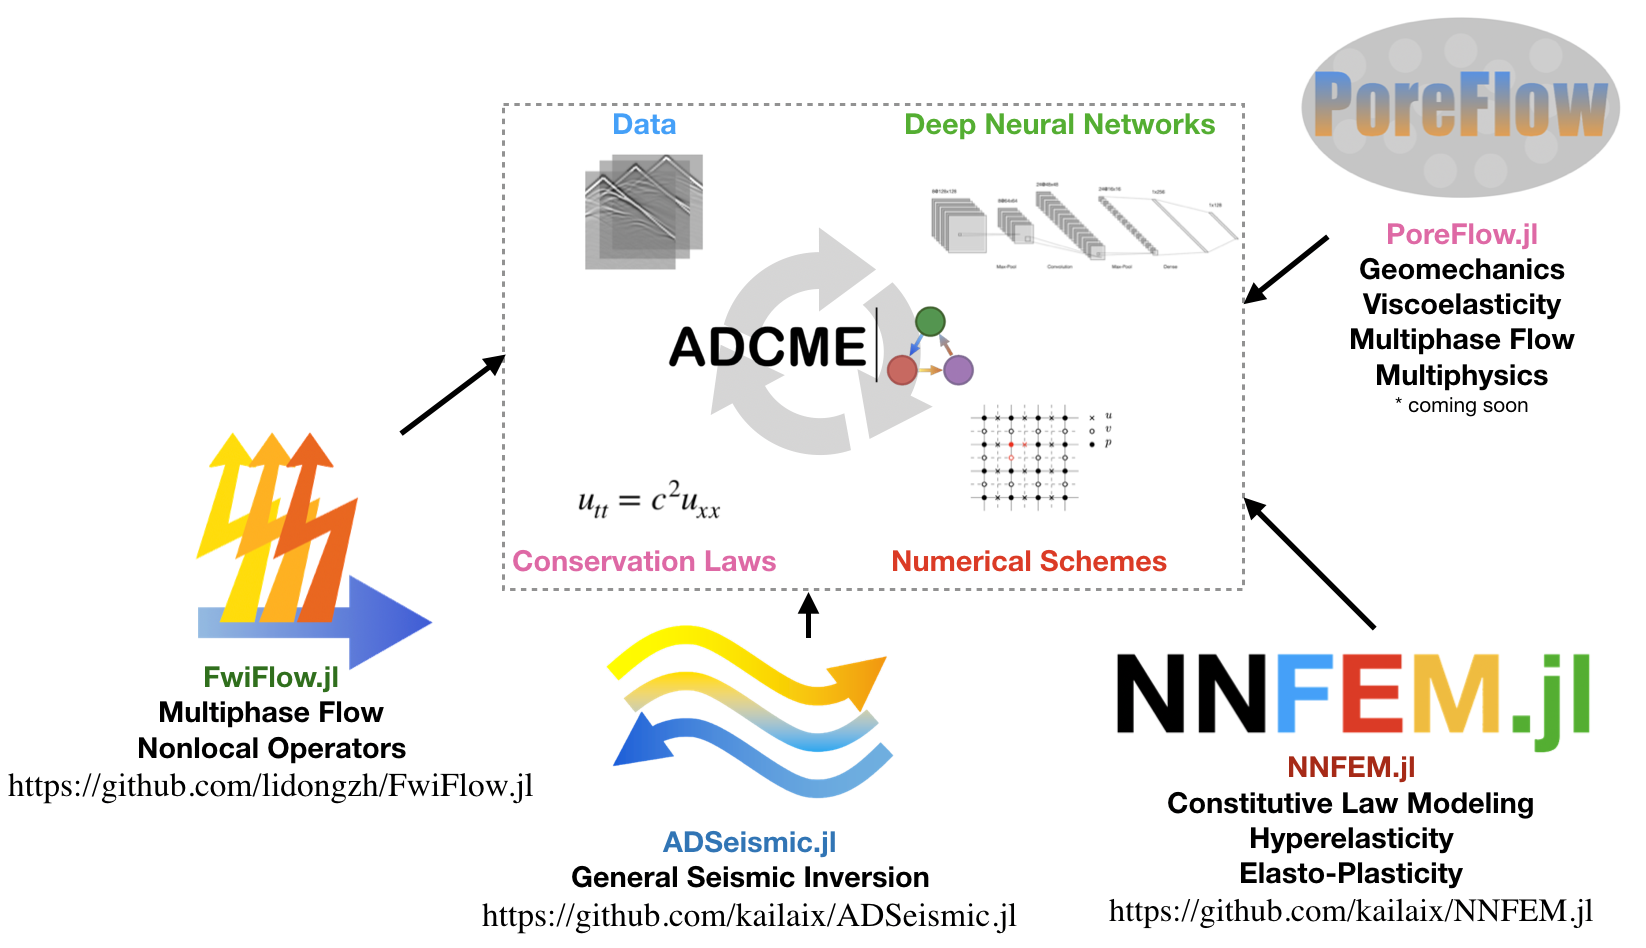
\includegraphics[width=1.0\textwidth]{figures/summary.png}
\end{figure}

\end{frame}




%}
%\usebackgroundtemplate{}
%----------------------------------------------------------------------------------------
%    PRESENTATION SLIDES
%----------------------------------------------------------------------------------------

%------------------------------------------------



\end{document} 